\documentclass[12pt]{amsart}
\usepackage{amsmath,amssymb}
\usepackage{geometry} % see geometry.pdf on how to lay out the page. There's lots.
\geometry{a4paper} % or letter or a5paper or ... etc
% \geometry{landscape} % rotated page geometry

%  POSSIBLY USEFULE PACKAGES
\usepackage{graphicx}
\usepackage{caption,subcaption}
\usepackage{tensor}
\usepackage[boxed,ruled]{algorithm2e}
\usepackage{todonotes}

%  NEW COMMANDS
\newcommand{\pder}[2]{\ensuremath{\frac{ \partial #1}{\partial #2}}}
\newcommand{\ppder}[3]{\ensuremath{\frac{\partial^2 #1}{\partial{align}
      #2 \partial #3} } }
\newcommand{\R}{\ensuremath{\mathbb{R}}}
\renewcommand{\H}{\ensuremath{\mathcal{H}}}
\newcommand{\norm}[1]{\ensuremath{\left\| #1 \right\| }}
\newcommand{\abs}[1]{\ensuremath{ | #1 | }}

%  NEW THEOREM ENVIRONMENTS
\newtheorem{thm}{Theorem}[section]
\newtheorem{prop}[thm]{Proposition}
\newtheorem{cor}[thm]{Corollary}
\newtheorem{lem}[thm]{Lemma}
\newtheorem{defn}[thm]{Definition}
\newtheorem{example}[thm]{Example}
\newtheorem{ass}{Assumption}

% NEW ENVIRONMENTS

%  MATH OPERATORS
\DeclareMathOperator{\Diff}{Diff}
\DeclareMathOperator{\Dens}{Dens}
\DeclareMathOperator{\SO}{SO}
\DeclareMathOperator{\U}{U}
\DeclareMathOperator{\B}{B}
\DeclareMathOperator{\Fr}{Fr}
\DeclareMathOperator{\OdeSolve}{OdeSolve}
\DeclareMathOperator{\Op}{Op}
\DeclareMathOperator{\Tr}{Tr}
\DeclareMathOperator{\card}{card}
\DeclareMathOperator{\Con}{Con}

%  TITLE, AUTHOR, DATE
\title{Qualitatively accurate spectral schemes for advection and transport}
\author{Henry O. Jacobs \& Ram Vasudevan}
\date{\today}


\begin{document}

\maketitle

\begin{abstract}
  blah blah blah.
\end{abstract}

%%%%%%%%%%%%%%%%%%%%%%%%%%%%%%%%%%%%%%%%%%%%%%%%%%%
\section{Introduction}
\label{sec:intro}

Let $M$ be a compact manifold and let $X$ be a vector-field on $M$. The current paper is concerned with the following two equations
\begin{align}
	\partial_{t} f + X^{i} \partial_{i} f = 0 \label{eq:function pde} \\
	\partial_{t} \rho + \partial_{t} (\rho X^{i}) = 0 \label{eq:density pde}
\end{align}
for a time dependent function $f$ and a time dependent density $\rho$ on $M$.
Both equations occur in a variety of contexts.
Equation \eqref{eq:function pde} describes how a scalar quantity (such as a particle label) is transported by the flow of $X$.
Such a pde arises in the context of fluids when $X$ is the (time-dependent) velocity field of the fluid, and $f$ is the temperature, and the thermal diffusivity is $0$.
In the context of imaging and computer vision, it is often desired that one evolve a surface under some prescribed dynamics.
For such a problem, level-set methods provide a possible numerical solution.
Level set methods begin by converting the surface into the level set of some function, $f$, and then solving \eqref{eq:function pde}.

Equation \eqref{eq:density pde} describes how a density (e.g. a probability distribution) is transported by the flow of $X$.
In the context of classical mechanics, this equation is known as the Louiville equation.
More generally, it can be seen as the zero-noise limit of the Fokker-Planck equation.
In the context of fluids, such an equation describes how the density of a chemical tracer is transported by $X$.

These equations have a number of conservation laws associated to them.
For example, if $f$ and $g$ are solutions to \eqref{eq:function pde},
then so is the product and the sum $f\cdot g$ and $f+g$.
Other such conservation laws will be described in a future section, but suffice it to say,
we will consider a numerical scheme to be qualitatively accurate if it exhibits a discretized version of these conservation laws. 

Both \eqref{eq:function pde} and \eqref{eq:density pde} can be approached, numerically, from a variety of directions, each with its own benefit.
For example, particle methods can be used, and do a decent job with regards to ``qualitative accuracy''.
The method of characteristics tells us that
the solution to \eqref{eq:function pde} with the initial condition $f_{0} \in C^{1}(M)$ is the time-dependent function $f( x_{t} ;t) = f_{0}( x_{0} )$ where $x_{t}$ is the solution to $\dot{x} = X(x)$.
This suggests the following numerical method for the case $M = S^{1}$.

\begin{algorithm} 
	\KwData{An initial function $f_{0}$ and a resolution $n$.}
	\KwResult{The value of the solution $f(x,t)$ to \eqref{eq:function pde} at time $t=1$ at a finite set of points.}.
	Initialize a regular grid $\{ x_{1},\dots,x_{n} \}$ on $S^{1}$\;
	\For{i = 1,\dots,n}{
		Solve the ode $\dot{x} = X(x)$ with final condition $x_{i}(1)$ using a method of choice (e.g. Euler's method)\;
	}
	\KwOut{ $f_{0}( x_{1}(0) ), \dots, f_{0}(x_{n}(0) )$. }
	\caption{The method of characteristics}\label{alg:particle}
\end{algorithm}
 
We will see that this algorithm retains many of the properties of \eqref{eq:function pde},
and we think it deserves the label of \emph{qualitatively accurate}.
For example, given the input $h_{0} = f_{0} \cdot g_{0}$, the output of Algorithm \ref{alg:particle} is identical to the componentwise product of the outputs obtained from inputing $f_{0}$ and $g_{0}$ separately.
In other words, Algorithm \ref{alg:particle} conserves a (discrete version of) multiplication of functions just like the original pde \eqref{eq:function pde}.
Moreover, this algorithm converges over finite time-intervals (using any reasonable interpolation method) at a rate $\mathcal{O}(n^{-1})$.
However, one drawback of this algorithm in the context of smooth data there exists algorithms which exhibit vastly superior convergence rates, namely spectral methods with spectral convergence.

In the case where $M=S^{1}$ a spectral method can be obtained by converting \eqref{eq:function pde} to the Fourier domain where it takes the form
of an ode
\begin{align}
	\frac{d \hat{f}_{k}}{dt} + 2\pi i \ell  \widehat{X}_{k-\ell} \hat{f}_{\ell} \label{eq:standard spectral}
\end{align}
where $\hat{f}_{k}$ and $\widehat{X}_{k}$ denote the Fourier transforms of $f$ and $X$.
We see that we have converted our linear pde into a linear ode on the space of Fourier coefficients.
A good numerical algorithm is obtained by considering only the first $2n+1$ such coefficients (see Algorithm \ref{alg:spectral}).

\begin{algorithm} 
	\KwData{An initial function $f_{0}$ and a resolution $n$.}
	\KwResult{A truncated Fourier series which approximates the solution $f(x,t)$ to \eqref{eq:function pde}, at time $t=1$.}
	Compute the Fourier expansion of $X = \hat{X}_{k} \exp( 2\pi i k)$ for $k=-n,\dots,0,\dots,n$\;
	Compute the Fourier expansion of $f_{0} = \hat{f}_{0,k} \exp( 2\pi i k)$ for $k=-n,\dots,0,\dots,n$\;
	Solve a truncated version of the linear system \eqref{eq:standard spectral} up to time $t=1$.\;
	\KwOut{$\hat{f}_{1,k}$ for $k= -n , \dots, 0 ,\dots,n$.}
	\caption{A standard spectral method for \eqref{eq:function pde}}\label{alg:spectral}
\end{algorithm}

Such a numerical method is good for smooth data, in the sense that the convergence rate is faster than $\mathcal{O}(n^{-p})$ for any finite $p > 0$ over a fixed finite time interval.
Such a convergence rate is known as \emph{spectral} or \emph{exponential}.
However, this algorithm is not qualitatively accurate.  It does not preserve sums and products of functions.

This motivates the primary goal of this paper:
to find a numerical algorithm for \eqref{eq:function pde} and \eqref{eq:density pde} which is spectrally convergent and qualitatively accurate.
From the previous discussion, it appears there are solutions to each of these goals individually, but not simultaneously.

\subsection{Previous work}
Papers to mention:
\begin{enumerate}
	\item \cite{HenrionKorda2014}
	\item Froyland, Koopman papers
	\item Representation theory stuff \cite{VershilGelfandGraev1975,Ismagilov1975}
	\item Naimark-Gelfand transform 
\end{enumerate}

%%%%%%%%%%%%%%%%%%%%%%%%%%%%%%%%%%%%%%%%%%%%%%%%%%%
\section{Qualitative properties of advection PDEs}
\label{sec:properties}
In this section we define specifically what we mean by ``advection PDEs'' in more precise mathematical terms.
Throughout this paper let $\mathfrak{X}(M)$ denote the space of smooth vector-fields on a compact manifold $M$
and let $X(t) \in \mathfrak{X}(M)$ be a time-dependent vector-field on $M$.
Let $\Phi^{t_{0},t_{1}}_{X}:M\to M$ denote the flow map of $X$ from time $t_{0}$ to $t_{1}$.
Given a bounded real-valued function $f_{0}$, we could consider the time-dependent function $f(x,t) := f_{0} ( (\Phi_{X}^{0,t})^{-1}(x) )$.
The function $f$ represents how $f_{0}$ is pushed and stirred around by the flow of $X$.
For a fixed $x \in M$ we observe, via the chain-rule,
\begin{align}
	 \frac{d}{dt}  f(x;t) &=  \left. \frac{d}{d \epsilon} \right|_{\epsilon=0} ( f(x;t+\epsilon) - f(x,t) ) \\
	 &=  \left. \frac{d}{d \epsilon} \right|_{\epsilon=0} \left( f( (\Phi_{X}^{t,t+\epsilon})^{-1}(x) , t ) - f(x,t) \right) \\
	 &=  \left. \frac{d}{d \epsilon} \right|_{\epsilon=0} \left( f(x,t) + \epsilon \pder{f}{x^{j}} [ (\Phi_{X}^{t,t+\epsilon})^{-1}(x) - x ]^{j} + \mathcal{O}(\epsilon^{2}) - f(x,t) \right) \\
	 &= - X^{j}(x) \pder{f}{x^{j}} = - \pounds_{X}[f_{0}]
\end{align}
where $\pounds_{X}[f]$ denotes the Lie-derivative of $f$.
This calculation yields the time-dependent advection PDE \eqref{eq:function pde}.

The same idea works if we consider the advection of a density $\rho_{0}$ by $X$.
In this case, the advected density is given by $\rho (x ; t) =  \det\left[ (D\Phi_{X}^{t,0})^{-1} (x) \right] \rho_{0}( (\Phi_{X}^{0,t})^{-1}(x) )$
and the advection PDE is \ref{eq:density pde}.

Similarly, a (constant in time) vector-field $Y_{0}$ is advected by $X$ by the formula $Y(x ; t) =  (D\Phi_{X}^{t,0})|_{(\Phi_{X}^{t,0})^{-1}(x)} \cdot Y_{0}( (\Phi_{X}^{t,0})^{-1}(x))$
and satisfies the advection PDE
\begin{align} \label{eq:vector field pde}
	\pder{Y^{i}}{t} + \pder{Y^{i}}{x^{j}} \cdot X^{j} - \pder{X^{i}}{x^{j}} \cdot Y^{j} = 0.
\end{align}

\section{Qualitative properties of advection}
\label{sec:properties}
Advection PDEs preserve a lot of natural structures.
For example if $f(x,t)$ and $g(x,t)$ are solutions to \eqref{eq:function pde}, then the scalar product $f(x,t) g(x,t)$  and the sum $f(x,t) + g(x,t)$ is also a solution to \eqref{eq:function pde}.
This observation can be summarized by the statement \emph{evolution by \eqref{eq:function pde} preserves the ring of functions on $M$}.
In the same vein, if $\rho$ is a density which satisfies \eqref{eq:density pde} and $f$ is a function which satisfies \eqref{eq:function pde}, then the quantity $c = \int_{M} f \cdot \rho$ is constant in time.
This can naturally be extended to the case where $\rho$ is a distribution, and we can summarize this conservation law by saying \emph{advection preserves the duality between functions and distributions on $M$}.

More conservation laws can be found for vector-field advection.
If $Y$ and $Z$ are vector-fields, then there is a natural Lie-bracket structure given by
\begin{align}
	[Y,Z]^{i} \equiv ( \pounds_{Y}[Z] )^{i} := \partial_{j}Z^{i} \, Y^{j} - \partial_{j}Y^{i} \, Z^{j}.
\end{align}
We can observe that if $Y$ and $Z$ satisfy \eqref{eq:vector field pde} then $[Y,Z]$ also satisfies \eqref{eq:vector field pde}.
In summary, advection preserves the Lie algebra of vector fields.

Lastly, the canonical relationships between vector-fields and functions and densities are also preserved.
Given a vector-field $Y$ a function $f$ and a density $\rho$ we may define the Lie derivatives
\begin{align}
	\pounds_{Y}[f] = Y^{j} \partial_{j}f \quad , \quad \pounds_{Y}[\rho] = \pder{}{x^{j}} ( \rho Y^{j} ).
\end{align}
The quantity $\pounds_{Y}[f]$ is itself a function, and $\pounds_{Y}[\rho]$ is a density.
If $f,\rho$ and $Y$ satisfy the advection PDEs \eqref{eq:function pde}, \eqref{eq:density pde}, and \eqref{eq:vector field pde} respectively,
then $\pounds_{Y}[f]$ satisfies \eqref{eq:function pde} and $\pounds_{Y}[\rho]$ satisfies \eqref{eq:density pde}.
In summary, advection preserves the action of vector fields on functions and densities.

In some sense these conservation laws are remarkable, since most PDEs do not conserve all the structures mentioned.
Of course, there is no such thing as magic.
The group of smooth diffeomorphisms of $M$ is in fact identical to the group of ring-automorphisms of $C^{\infty}(M)$.
The formal Lie algebra of the group of Diffeomorphisms is the space of vector-fields $\mathfrak{X}(M)$.
So it is no wonder that advection preserves the ring-structure of functions.
Moreover, the space of distributions is \emph{defined} as the dual space to that of functions, and so the action of a vector-field on distributions is defined
as the dual of the action on functions.
So of course advection preserves the duality between functions and distributions.
Lastly, any Lie group preserves it's own Lie algebra and its own group actions.
So of course advection preserves the Lie bracket of vector fields and the Lie derivatives of functions and densities.
These conservation laws are fundamental properties of advection, and this motivates the definition of qualitative accuracy
which we shall use in this paper:

\begin{center}
    \fbox{
    	\begin{minipage}{0.8\textwidth}
    		A numerical method for an advection is {\bf qualitatively accurate} if it conserves (up to machine precision) the same properties as the exact advection PDE.
    	\end{minipage}
    }
\end{center}

This criterion is separate from numerical accuracy, and can be evaluated independently.
Of course, numerical accuracy takes first priority,
but the goal of this paper will be to go the extra length of constructing a scheme which is numerically
\emph{and qualitatively} accurate.

%%%%%%%%%%%%%%%%%%%%%%%%%%%%%%%%%%%%%%%%%%%%%%%%%%%
\section{The canonical space $L^{2}(M)$}
\label{sec:half densities}
The goal of this paper is to construct a spectral advection scheme which exhibits a large number of invariants.
At the core of many spectral schemes is the use of some Hilbert space upon which everything can be approximated via least squares projections.
Typically this Hilbert space is $L^{2}(M ; \mu)$ where the $L^{2}$-inner product is taken with respect to some non-canonical density or volume form $\mu$ on $M$.
We do not have this luxury.
The properties of advection that we desire to have are strictly properties of $M$ alone, i.e. they are canonical.
Any non-canonical choices we make in constructing our scheme (such as the choice of a volume form) threaten to break these conservation laws by introducing non-canonical artifacts.

In this section we define a geometric version of an $L^{2}$-space which foregoes the choice of a volume form, denoted simply by $L^{2}(M)$.
The ``cost'' we pay for not choosing a volume form is that the elements of $L^{2}(M)$ are not (equivalence classes of) functions because they transform differently under a change of coordinates.

Again, let $M$ be a smooth compact $n$-manifold
and we will let $\Dens(M)$ denote the space of continuous densities,
which we view as anti-symmetric multilinear functions on $\bigoplus^n TM$ \cite[Chapter 16]{Lee2006}.

\begin{defn}\label{def:half density}
	A half-density is a continous complex function $\psi : \bigoplus^n TM \to \mathbb{C}$
	such that $| \psi |^{2} \in \Dens(M)$.
	We denote the space of half densities by $\sqrt{\Dens(M)}$.
\end{defn}

This definition is an equivalent reformulation of the half densities defined in the context of geometric quantization \cite{GuilleminSternberg1970,BatesWeinstein1997}.
In physical terms, $L^{2}(M)$ is precisely the Hilbert space of wave functions on $M$ used in quantum mechanics.
It is unfortunate that physicists call these ``wave-functions''
because elements of $L^{2}(M)$ and $\sqrt{\Dens(M)}$ are \emph{not} functions on $M$.\footnote{However, this sloppy use of names is consistent with others instances such as the fact that the ``Dirac-delta function'' is also not a function.}
One way to see this is to observe how elements of $\sqrt{\Dens(M)}$ transform.
Under a change of coordinates $\Phi$ we observe $\psi$ will map to $\tilde \psi$ where
\begin{align}
	\tilde{\psi}(x)  =  \left| \det \left[ \left. \pder{\Phi^{i}}{x^{j}} \right|_{\Phi^{-1}(x)} \right]_{i,j=1}^{n} \right|^{1/2} \psi( \Phi^{-1}(x) ). \label{eq:transformation law}
\end{align}


As $|\psi|^{2} \in \Dens(M)$ for any $\psi \in \sqrt{\Dens(M)}$ we can integrate $|\psi|^{2}$
and observe that half densities are is naturally equipped with the norm $$\| \psi \|_2 :=  \left( \int_M |\psi|^2 \right)^{1/2}$$ which we call the $2$-norm.

\begin{defn}
	We define $L^{2}(M)$ as the completion of $\sqrt{ \Dens(M)}$ with respect to the $2$-norm.
	The space $L^{2}(M)$ is equipped with a complex inner-product given by
	\begin{align}
		\langle \psi \mid \phi \rangle = \int_{M} \bar \psi \phi
	\end{align}
	through polar decomposition, and so $L^{2}(M)$ is a Hilbert space.
\end{defn}

Lastly, as we know how to transform half-densities, we also know how to advect them.
For a vector-field $X$, the Lie derivative of a half-density is given in local coordinates by
\begin{align}
	\pounds_{X}[\psi] = \frac{1}{2} X^{i} \pder{\psi}{x^{i}} + \frac{1}{2} \pder{}{x^{i}} \left( \psi X^{i} \right). \label{eq:half density pde}
\end{align}
This is an unbounded anti-Hermetian operator on $L^{2}(M)$.
The advection equation can be written as
\begin{align}
	\partial_{t} \psi + \pounds_{X}[\psi] = 0.
\end{align}
By the Stone Von-Neumann theorem \cite{Conway1990}, there is a solution for all time, in spite of the fact that the Lie derivative is an unbounded operator.
Moreover, the solution is given by a unitary action.  For reference later, we restate this remark formally.
\begin{prop} \label{prop:stone}
	The solution to \eqref{eq:half density pde} is of the form $\psi(t) = U(t) \cdot \psi(0)$ where $U(t)$ is
	the unitary operator.
\end{prop}
%\begin{proof}
%	Again, the existence of $U(t)$ as a unitary operator is simply an instance of the Stone Von-Neumann theorem.
%\end{proof}

In fact, $U(t)$ is merely the push-forward operator given in \eqref{eq:transformation law} with ``$\Phi$'' replaced by the flow-map of the dynamics.
We will generally avoid using this explicit expression though, as it can be cumbersome.


\subsection{The relationship with classical $L^{2}$ spaces}
\label{sec:classical_Lebesgue}
For any manifold $M$ (possibly non-orientable) one can assert the existence of a smooth non-negative density $\mu$.
Upon choosing some $\mu$, the $2$-norm of a complex function $f$ with respect to $\mu$ is
\begin{align}
	\| f \|_{\mu,2} =  \left( \int_M |f|^2 \mu \right)^{1/2}.
\end{align}
and $L^2(M ; \mu)$ is the completion of the space of continuous functions with respect to this norm.
The relationship between $L^{2}(M)$ and $L^{2}(M;\mu)$ is that they are identical as topological vector-spaces.
In fact, the isomorphism can be given fairly explicitly.

\begin{prop}
	Choose a non-vanishing density $\mu$.
	Let $\sqrt{\mu}$ be any half-density such that $| \sqrt{\mu} |^{2} = \mu$.
	For any $\psi \in L^2(M)$ there exists a unique $f \in L^2(M ; \mu)$ such that $\psi = f \cdot  \sqrt{\mu}$.
	This yields a continuous isomorphism between $L^2(M)$ and $L^2(M ; \mu)$.
\end{prop}
%\begin{proof}
%	First note that if we view $\mu$ as a positive function on $\bigoplus^n TM$, then we can simply set $\sqrt{\mu}$ to be it's classical square root.
%	It suffices to prove that the dense subspace $\sqrt{\Dens(M)} \subset L^{2}(M)$ can be mapped to a dense subspace of $L^{2}(M;\mu)$ through a map that sends $\| \cdot \|_{2}$ to $\| \cdot \|_{\mu,2}$.
%	
%	Let $\psi \in \sqrt{\Dens(M)}$.  Then $|\psi|^2$ is a continuous density.
%	The Radon-Nikodym derivative of $|\psi|^{2}$ with respect to $\mu$ is a positive valued continuous function $g \in C^0(M)$ defined such that $g \, \mu = |\psi|^2$.
%	Without loss of generality, we may set $g = |f|^{2}$ for some complex function $f$ such that $\psi = f\, \sqrt{\mu}$.
%	The function $f$ is unique with respect to $\psi$ and
%	the map $\psi \in \sqrt{\Dens(M)} \mapsto f \in C^0(M ; \mathbb{C} )$ sends $\| \cdot \|_{2}$ to $\| \cdot \|_{\mu,2}$ by construction.
%	Thus the map is continuous.
%	The inverse of the map is given by $f \in C^{0}(M;\mathbb{C}) \mapsto f \, \sqrt{\mu} \in \sqrt{\Dens(M)}$.
%\end{proof}

At this point the reader might ask ``If both space are the same, then why don't we use the one that is more familiar?  i.e. the space $L^{2}(M;\mu)$''.
The answer is that these space are really not the same in all aspects.
One difference that we've already discussed is that they transform differently.
Elements of $L^{2}(M)$ transform according to \eqref{eq:transformation law} while elements of $L^{2}(M;\mu)$ transform like functions.
Additionally, a more useful difference for us is that $L^{2}(M)$ is \emph{not} contained within $L^{1}(M)$ and $L^{\infty}(M)$ is not contained in $L^{2}(M)$
because each of these spaces consists of objects with different transformation properties.
This separation between $L^{2}(M)$ and $L^{1}(M)$ \emph{forces} us to think of these objects as distinct.
For example an operator on $L^{2}(M)$ can not generally be applied to $L^{1}(M)$ in the same way.
Later we will find this is a good thing, because it allows us to have an operator act on $L^{1}(M)$ differently than how it acts on $L^{2}(M)$
without leading to contradiction.
Such safety mechanisms are analogous to the use of private/public functions in object oriented programming, which place constraints on a computer program in order to banish certain bugs from arising.

\subsection{Sobolev spaces}
\label{sec:Sobolev spaces}
For each $X \in \mathfrak{X}(M)$ the operator $\pounds_{X}$ on $L^{2}(M)$ is unbounded.
In the parlance of functional analysis, the domain of $\pounds_{X}$ is
\begin{align}
	\operatorname{dom}( \pounds_{X} ) := \{ \psi \in L^{2}(M) \mid  \| \pounds_{X}[\psi] \|_{L^{2}} < \infty \}.
\end{align}
One can then show that $\operatorname{dom}( \pounds_{X} )$ is a closed subspace of $L^{2}(M)$ and then define
a \emph{canonical} Sobolev space
\begin{align}
	H^{1}(M) := \bigcap_{X \in \mathfrak{X}(M)} \operatorname{dom}( \pounds_{X} ).
\end{align}
Where we view $\pounds_{X}$ as an unbounded operator on $L^{2}(M)$.
More generally, we can construct $H^{k}(M)$ by composing multiple Lie derivative operators,
and we can even consider fraction degrees of regularity as well.
%As $\pounds_{X}$ is anti-Hermetian we can invoke the spectral theorem of functional analysis
%and consider the operator
%\begin{align}
%	(\pounds_{X})^{s} [ \psi] = \sum_{\lambda \in \sigma( \pounds_{X}) } \lambda^{s} \langle e_{\lambda} \mid \psi \rangle e_{\lambda}
%\end{align}
%where $\{ e_{\lambda} \mid \lambda \in \sigma( \pounds_{X}) \}$ denotes the set of eigenvectors of $\pounds_{X}$. 
%This fractional power of $\pounds_{X}$ allows us to consider Sobolev spaces of fractional orders as well.

  However, while the canonicalism of $L^{2}(M)$ will be quite useful to us,
  \emph{canonical} (metric-free) Sobolev spaces will not be.
  We will find that our algorithms only converge on spaces of sufficient regularity,
  but in order to perform our error-analysis we will need to choose a non-canonical norm.
  
To begin the process of choosing a norm for $H^{s}(M)$, equip $M$ with a Riemannian metric $g:TM \oplus TM \to \mathbb{R}$.
The metric induces a positive density $\mu_g$,
known as the \emph{metric density}. 
The Riemmanian density induces the $L^2$ inner-product on $C^\infty(M)$ via
\begin{align}
	\langle f_1 , f_1 \rangle_{g} = \int \overline{f_1} \cdot f_2 \mu_g
\end{align}
and $L^{2}(M;\mu_{g})$ is the completion of the inner-product space $( C^{\infty}(M) , \langle \cdot , \cdot \rangle_{g})$ under 
the inner-product norm.
The metric also induces an elliptic operator, known as the Laplace-Beltrami operator $\Delta: C^{\infty}(M) \to C^{\infty}(M)$, which is is positive-semidefinite
with respect to $\langle \cdot , \cdot \rangle_{g}$.
If $M$ is compact, then $L^2(M ; \mu_g) \cong L^2(M)$ is a separable Hilbert space
and the Helmholtz operator, $1 + \Delta$, is then a positive definite operator
with a discrete spectrum.
For any $s \geq 0$ we may define the Sobolev norm
\begin{align}
	\| f \|_{s,2} =  \left( \langle f , (1+\Delta)^s \cdot f \rangle_{g} \right)^{1/2}
\end{align}
and $H^s(M ; g)$ is then the function space obtained by completion with respect to this norm, and modulo discrepancies of measure zero.
Note that $H^0(M;g) = L^2(M;\mu_g)$.

The following proposition will be of use later when we need to prove a notion of convergence
via sequences of finite rank operators.

\begin{prop} \label{prop:compact_embedding}
	Let $(M,g)$ be a compact Riemmanian manifold.  If $s > t \geq 0$ then $H^s(M;g)$ is compactly embedded within $H^t(M,g)$.
\end{prop}
\begin{proof}
	As $M$ is compact we know that the spectrum of $\Delta$ is discrete and $L^{2}(M)$ is separable.
	Let $e_0, e_1,\dots$ be the Hilbert basis for $L^2(M;\mu_g)$ which diagonalizes $\Delta$
	in the sense that $\Delta e_i = \lambda_i e_i$ for a sequence $0 = \lambda_0 \leq \lambda_1 \leq \lambda_2 \leq \cdots$.
	The operator $(1+\Delta)^s$ is given by
	\begin{align}
		(1+\Delta)^s \cdot f =  \sum_{i} e_i (1+\lambda_i)^s \langle e_i , f \rangle_g,
	\end{align}
	and so $\{ (1+ \lambda_i)^{-s} e_i \}_{i=1}^{\infty}$ is a Hilbert basis for $H^s(M;g)$.
	
	Let us call $e_i^{(s)} = (1+ \lambda_i)^{-s} e_i$.
	The embedding of $H^s(M;g)$ into $H^t(M,g)$
	is then given in terms of the respective basis elements by $e_i^{(s)} \mapsto (1+\lambda_i)^{-(s-t)}e_i^{(t)}$.
	As $s > t$ and $\lambda_i \to +\infty$, we see that 
	this embedding is a compact operator \cite[see Proposition 4.6]{Conway1990}.
\end{proof}

In the sequel we shall say that $\psi \in L^2(M)$ is of class $H^s$ if $\psi = f \sqrt{\mu_g}$, and $f \in H^s(M,g)$.
That $\psi$ is of class $H^{s}$ is topological statement, and not metric dependent.
However, the norm $\| \psi \|_{2,s} = \| f \|_{2,s}$ is metric dependent.

\section{A spectral discretization}
The goal of this section will be to produce a spectral scheme for the advection equations \eqref{eq:function pde}, \eqref{eq:density pde}, and \eqref{eq:vector field pde}
using the space $L^{2}(M)$.
In order to realize this goal we must relate functions, densities, and vector-fields to $L^{2}(M)$ in a way that can be spectrally discretized without breaking any canonical structures.

To begin, let us consider the space of continuous real-valued functions $C(M)$.
For each $f \in C(M)$ there is a unique bounded Hermetian operator, $\hat{f} : L^{2}(M) \to L^{2}(M)$ given by scalar multiplication.
That is to say $(\hat{f} \cdot \psi) (x) = f(x) \psi(x)$.
We see that the hat-map, $f \mapsto \hat{f}$, preserves the ring structure because $\widehat{f \cdot g + h} = \hat{f} \cdot \hat{g} + \hat{h}$.

Similarly, (and in the opposite direction) for any trace class operator $\hat{\rho}$ there is a unique distribution $\rho \in C(M)'$ such that 
\begin{align}
	 \int f \, \rho = \Tr ( \hat{f}^{\dagger} \cdot \hat{\rho} )
\end{align}
for any $f \in C(M)$.
By construction, the surjection $\hat{\rho} \mapsto \rho$ and the injection $f \mapsto \hat{f}$ preserve the duality between functions and distributions.

Finally, for any vector field $X$ there is a unique (unbounded) anti-symmetric operator $\pi(X)$ on $L^{2}(M)$
given in coordinates by
\begin{align}
	\pi(X) \cdot \psi = \frac{1}{2} X^{j} \pder{\psi}{x^{j}} + \frac{1}{2} \pder{}{x^{j}} ( \psi \, X^{j} ). \label{eq:representation}
\end{align}
After some minor computations (see Appendix \ref{app:Lie} \todo{need to write an appendix} ) we see that $\pi$ is a Lie algebra morphism which sends
the Jacobi-Lie bracket to (minus) the commutator bracket.  That is to say, $\pi$ is linear and $\pi([X,Y]) = - [ \pi(X) , \pi(Y)]$.

\begin{example}
Let us describe what this means when $M$ is a torus.
In standard coordinates $\theta = (\theta^{1},\dots,\theta^{d})$ we may write $X = X^{i}(\theta) \frac{\partial}{\partial \theta^{i}}$ for some functions $X^{1}(\theta),\dots,X^{d}(\theta)$.
In a Fourier basis $\{ \frac{1}{\sqrt{2\pi}} e^{ i \langle k , \theta \rangle}   \mid k \in \mathbb{Z}^{d} \}$ 
a half density, $\psi$ is given by it's Fourier series $\mathcal{F}[\psi]$.
Upon noting that $\mathcal{F}[ f \cdot \psi] = \mathcal{F}[f] * \mathcal{F}[\psi]$
we find $\hat{f} = \mathcal{F}[f] * $, i.e. $\hat{f}$ is the convolution operator associated to the Fourier transform of $f$.
We observe that $\pi \left( \pder{}{\theta^{j}} \right) \cdot e^{i \langle k , \theta \rangle}  = i k^{j} e^{i \langle k,\theta\rangle}$.
That is to say, $\pi \left( \pder{}{\theta^{j}} \right)$ simply multiplies the $k$th mode by $k^{j}$.
This is the sparsest representation of this operator one can ever expect to obtain.
We then see that $\pi(X) \cdot \psi = \mathcal{F}[X^{j}] *  [ \pi \left( \pder{}{\theta^{j}} \right) \cdot \psi ]$.
If $X$ is smooth, than $\mathcal{F}(X^{j})$ is well approximated by a sparse operator by truncation.
As a result, we have a sparse spectral approximation of $\pi(X)$ when we use truncation.

Finally, given a sufficiently regular\footnote{e.g. $W^{1+\epsilon,1}$ for $\epsilon >0$ will do.} density, $\rho$,  we could 
split $\rho$ into non-negative and non-positive components as $\rho = \rho^{+} - \rho^{-}$
so that $\psi = \sqrt{\rho^{+}} + i \sqrt{\rho^{-}}$ is a square root of $\rho$.
Then $\hat{\rho}$ is represented in the Fourier domain by $\mathcal{F}(\psi) \otimes \mathcal{F}(\psi)^{\dagger}$.
\end{example}

We can now convert the evolution PDEs \eqref{eq:function pde}, \eqref{eq:density pde}, and \eqref{eq:vector field pde}
into ODE's of operators on $L^{2}(M)$.

\begin{thm} \label{thm:quantize}
	Let $X(t) \in \mathfrak{X}(M)$ be a time-dependent vector-field.
	Then $f$, $\rho$, and $Y$ satisfy \eqref{eq:function pde},\eqref{eq:density pde}, and \eqref{eq:vector field pde} respectively
	if and only if $\hat{f}$, $\hat{\rho}$, and $\pi(Y)$ satisfy the operator ODEs
	\begin{align}
		&\frac{d \hat{f} }{dt} + [ \hat{f} , \pi(X) ] = 0 \label{eq:quantum observable ode} \\
		&\frac{d \hat{\rho} }{dt} + [ \hat{\rho} , \pi(X) ] = 0 \label{eq:quantum density ode} \\
		&\frac{d \pi(Y) }{dt} + [ \pi(Y), \pi(X) ] = 0 \label{eq:quantum vf ode}
	\end{align}
	respectively.
	Moreover, if $\psi \in L^{2}(M)$ is such that $\psi^{2} = \rho$ and $\psi$ satisfies \eqref{eq:half density pde}, then $\rho$ satisfies \eqref{eq:density pde}.
\end{thm}

\begin{proof}
	Let $f$ satisfy \eqref{eq:function pde}.
	For an arbitrary $\psi \in L^{2}(M)$ we observe that $[ \hat{f} , \pi(X)] \cdot \psi$ is given in coordinates by
	\begin{align}
		[ \hat{f} , \pi(X) ] \cdot \psi = f \left( \frac{1}{2} X^{j} \pder{\psi}{x^{j}} + \frac{1}{2} \pder{}{x^{j}} ( \psi \, X^{j} ) \right)
			- \frac{1}{2} X^{j} \pder{}{x^{j}}( f \psi)  + \frac{1}{2} \pder{}{x^{j}} (f \psi \, X^{j} )
	\end{align}
	where we have used \eqref{eq:representation}.  Application of the product rule to all these terms then yields
	a number of cancellations and we find
	\begin{align}
		[ \hat{f} , \pi(X) ] \cdot \psi = - X^{j} \pder{f}{x^{j}} \psi = (\partial_{t} f )\psi = \frac{d \hat{f} }{dt} \cdot \psi.
	\end{align}
	As $\psi$ is arbitrary we have managed to show that $\hat{f}$ satisfies \eqref{eq:quantum observable ode}.
	Each line of reasoning is reversible, and so we have proven the converse as well.
	
	In order to handle densities note that $\langle f , \rho \rangle = \int_{M} f\rho$ is constant in time when $f$
	and $\rho$ satisfy \eqref{eq:function pde} and \eqref{eq:density pde} respectively.
	By the definition of $\hat{\rho}$ we observe $\Tr( \hat{f}^{\dagger} \hat{\rho}) = \langle f , \rho \rangle$.
	Thus we find
	\begin{align}
		0 = \frac{d}{dt} \left( \Tr( \hat{f}^{\dagger} \rho ) \right) = \Tr \left( \frac{d \hat{f}^{\dagger}}{dt} \hat{\rho} + \hat{f}^{\dagger} \frac{d \hat{\rho}}{dt} \right).
	\end{align}
	As was just shown, $\frac{d}{dt} \hat{f} =  - [\hat{f} , \pi(X) ]$ so we observe
	\begin{align}
		0 = \Tr( - [\hat{f} , \pi(X) ]^{\dagger} \hat{\rho} + \hat{f}^{\dagger} \hat{\rho} ) = \Tr( - \pi(X)^{\dagger} \hat{f}^{\dagger} \hat{\rho} + \hat{f}^{\dagger} \pi(X)^{\dagger} \hat{\rho} + \hat{f}^{\dagger} \frac{d\hat{\rho}}{dt} ).
	\end{align}
	Upon noting that $\pi(X)^{\dagger} = - \pi(X)$ and use of identity $\Tr( a b c) = \Tr( bc a)$ we obtain
	\begin{align}
		0 = \Tr \left( \hat{f}^{\dagger}( [\hat{\rho} , \pi(X) ] + \frac{d \hat{\rho}}{dt} ) \right).
	\end{align}
	As $\hat{f}$ was chosen arbitrarily, the desired result follows.
	Again, this line of reasoning is reversible.
	
	Thirdly, if $Y$ satisfies \eqref{eq:vector field pde}, then we observe 
	\begin{align}
		\frac{d}{dt} \pi(Y) = \pi ( \partial_{t} Y ) = \pi( - [X,Y] ) = [\pi(X) , \pi(Y) ].
	\end{align}
	where we have used the fact that $\pi$ is bracket preserving.
	
	Lastly, if $\psi$ satisfies \eqref{eq:half density pde} and $\rho = \psi^{2}$ then we see
	\begin{align}
		\partial_{t} \rho &= \partial_{t} ( \psi^{2}) = 2 (\partial_{t} \psi ) \, \psi \\
		&= 2 \left( - \frac{1}{2} \partial_{i} (\psi X^{i}) - \frac{1}{2} X^{i} \partial_{i} \psi \right) \psi \\
		&= \left( - X^{i} \partial_{i} \psi - \psi \partial_{i} X^{i}  \right) \psi \\
		&= - 2 \psi (\partial_{i} \psi) X^{i} - (\partial_{i}X^{i}) \psi^{2}\\
		&= - \partial_{i}(\rho) X^{i} - (\partial_{i}X^{i}) \rho = - \partial_{i} ( \rho X^{i}).
	\end{align}
\end{proof}


The benefit of representing our pde's in the form \eqref{eq:quantum observable ode},\eqref{eq:quantum density ode}, and \eqref{eq:quantum vf ode}
is that we may \emph{canonically} discretize these ODEs using least squares projections.  In order to demonstrate this, we will illustrate a detailed implementation of how this would be done on the unit circle, $S^1$, before considering the case of a general compact manifold.

\subsection{Discretization on $S^1$ using the Fourier Transform}
In the case of $S^1$ we can discretize all the needed concepts using the Fourier transform.  In particular, let us consider the ODE $\dot{x} = g(x)$ where
$g(x)$ is a continuous function of $x \in S^1$.
Then the operator $\pi(X)$ is given by
\begin{align}
	\left( \pi(X) \cdot \psi \right)(x) = \frac{1}{2}
	\left( g(x) \left.\frac{d\psi}{dx}\right|_x 
	+ \left. \frac{d}{dx} \right|_x (g \cdot \psi ) \right). \label{eq:S1 op}
\end{align}

We will first describe how one can approximate the operator $\pi(X)$ with an operator on $\mathbb{C}^{2n+1}$ for a finite $n > 0$.
In essence what we will describe is a standard spectral scheme \cite{Boyd2001,NumericalRecipes}.
To begin, note that $\pi(X)$ consists of either multiplication by $g(x)$, or differentiation, or multiplication by $1/2$.  So our approach will be to discretize the linear operations of multiplication by $g(x)$ and the linear operation of differentiation.

The first step is to transform everything to the Fourier domain.  Any $\psi \in L^2(M)$ can be viewed as a normal $L^2$-function with respect to the standard Haar measure on $S^1$.  We may then apply the Fourier transform to write $\psi$ as a complex series
\begin{align}
	\psi(x) = \sum_{k=-\infty}^\infty c_k e^{2\pi i k x}.
\end{align}
We find that differentiation takes the form
\begin{align}
	\frac{d}{dx} (\psi)(x) = \sum_{k} 2\pi i k c_k e^{2\pi i kx}.
\end{align}
Thus, in the Fourier domain, differentiation is given by
\begin{align}
 	c_k \mapsto 2 \pi ik c_k
\end{align}
for all $k \in \mathbb{Z}$.
For any $N \in \mathbb{N}$ we may approximate the differentiation operator with a complex matrix
\begin{align*}
	[D_N]_{k \ell } = \delta_{k \ell } 2\pi i k
\end{align*}
for $k,\ell \in \{ -N , \dots,-1,0,1,\dots N \}$.
If we define $\mathbf{c}_n = ( c_{-n}, \dots , c_{-1} , c_0 , c_{1},\dots,c_n ) \in \mathbb{C}^{2n+1}$, the vector $D_n \cdot {\bf c}_n$ is the truncated Fourier series of $\frac{d\psi}{dx}$.

Similarly we may take the Fourier transform of the function $g$ to get the Fourier series expansion
\begin{align}
	g(x) = \sum_k g_k e^{2\pi i kx}.
\end{align}
Multiplication of $\psi \in L^2(S^1)$ by $g \in C^0(M)$ is given by
\begin{align}
	g(x) \cdot \psi(x) &= \sum_{k \ell} g_\ell c_k e^{2\pi i (k+\ell)x} \\
		&= \sum_{k \ell} g_{k-\ell} c_k e^{2\pi i kx}.
\end{align}
In other-words, the multiplication operator $\hat{g}$ is nothing but the convolution operator
\begin{align}
	( \hat{g} \cdot \psi )(x) = \sum_{k \ell} g_{k-\ell} c_k e^{2\pi i kx}.
\end{align}

Again, we can approximate $\hat{g}$ with a complex $(2N+1) \times (2N+1)$ matrix
\begin{align}
	[\hat{G}_N]_{k\ell} = g_{k - \ell}
\end{align}
for $k,\ell \in \{ -N , \dots,-1,0,1,\dots,N\}$.
We will find that $\hat{G}_N$ converges to $\hat{g}$ as $n$ goes to infinity.
As a result the matrix-vector computation
\begin{align}
	 {\bf d}_N = {\bf X}_N \cdot {\bf c}_N
\end{align}
where
\begin{align}
	{\bf X}_N = \frac{1}{2} \hat{G}_N \cdot D_N + \frac{1}{2} D_N \cdot \hat{G}_N
\end{align}
serves as an approximation of the truncated Fourier series to \eqref{eq:S1 op}.
We will see that this approximation converges to order $\mathcal{O}( N^{1-s} )$ on the subspace $H^{s} \subset L^{2}$.

This gives us the following numerical scheme for \eqref{eq:half density pde} for a fixed $n$:

\begin{enumerate}
	\item Given the initial condition $\psi(0) \in L^2(S^1)$ compute ${\bf c}_N(0)$.
	\item Solve the ode $\frac{d {\bf c}_N }{dt} = {\bf X}_N \cdot {\bf c}_N$ over a finite time interval, $[0,T]$,
	with a trusted ode solver.\footnote{If ${\bf X}_n$ is constant in time, than one can solve this ode using a matrix exponential, but this could be treacherous
	and needlessly expensive \cite{Moler2003}.}
	\item Let $\psi_{N}(x,t) = \sum_{k=-N}^N c_k(t) e^{2\pi ikx}$. 
\end{enumerate}
We will later find that $\psi_{N}$ converges to the solution of \eqref{eq:half density pde} at a rate $\mathcal{O}( N^{1-s})$ when $\psi(0) \in H^{s}(M)$ for $s > 1$.
Moreover, we will find that $\rho^{(n)} = ( \psi^{(n)} )^2$ converges to solutions of \eqref{eq:density pde} at the same rate.

Lastly, we can approximate solutions to \eqref{eq:function pde}
by discretizing \eqref{eq:quantum observable ode} in a similar way.
Given an initial condition $f(x,0) \in C^0(M)$ we can compute the truncated Fourier series $f_{-n},\dots,f_{-1},f_0,f_1,\dots,f_n$ and create the convolution matrix
\begin{align*}
	[ \widehat{F}_n(0) ]_{k \ell} = f_{k-\ell}.
\end{align*}
Again, $\widehat{F}_n(0)$ is a truncated approximation of the operator $\widehat{f( \cdot , 0)}$.
We then can approximate a solution to \eqref{eq:quantum observable ode}
 by integrating the finite-dimensional matrix ode
\begin{align*}
	\frac{d \widehat{F}_n }{dt} + [ \widehat{F}_n , {\bf X}_n ] = 0.
\end{align*}

Conversion of the matrix $\widehat{F}_n$ is admittedly a problem with this approach.  Another problem with this approach is the potential storage cost.

\subsection{Numerical algorithms on compact manifolds}

In this section will will present numerical algorithms for solving \eqref{eq:function pde} and \eqref{eq:density pde} given a vector field $X \in \mathfrak{X}(M)$.
The basic ingredient for all the algorithms in this section is a Hilbert basis and an ode solver.
We will denote the Hilbert basis by $\{ e_{0}, e_{1},\dots \}$ for $L^{2}(M)$.
For example we may choose a Riemannian metric, $g$, and let $\{ f_{0}, f_{1},\dots \}$ denote  eigen-functions of the Laplace operator.
Then $\{ e_{k} = f_{k} \sqrt{\mu_{g}} \mid k \in \mathbb{N} \}$ forms a smooth Hilbert basis for $L^{2}(M)$ where $\mu_{g}$ denotes the Riemmannian density.
In order to ensure convergence we will assume
\begin{ass} \label{ass:basis}
	There exists a metric such that the unitary transformation, $U:L^{2}(M) \to L^{2}(M)$, which sends the basis $\{ e_{k} \}$ to the Fourier basis $\{E_{k} \}$
	is bounded on $H^{s}$ for some $s > 1$.
\end{ass}
The above assumption holds for a variety of choices, such as the Fourier basis itself, as well as any Sturm-Louiville basis (e.g. Legendre functions, sufficiently regular wavelets, etc.).

For the ode solver, one can consider any legacy method such as Euler's method or 4th order Runge-Kutta or even well tested software such as \cite{VODE}.
This article is concerned purely with the semi-discretization of \eqref{eq:function pde} and \eqref{eq:density pde}, and so we will assume that this ode solver 
efficiently solves finite dimensional ODEs to any prescribed accuracy.
More explicitly, we will let $\OdeSolve ( F , x_{init} , t_{final} )$ denote $x(t_{final})$ when $x(t)$ is the solution to the ode $\dot{x} = F(x)$ with initial condition $x_{init}$.

Before solving \eqref{eq:function pde} and \eqref{eq:density pde}, let us solve \eqref{eq:half density pde} using a standard spectral discretization \cite{Boyd2001,NumericalRecipes}.

\begin{algorithm}
	\KwData{An initial condition $\psi(0) \in L^{2}(M)$, an ordered sequence of times $0 < t_{1} < t_{2} < \dots < t_{m}$, and a positive integer $n$.}
	\KwResult{A numerical solution, $\psi_{n}(t_{k})$, to \eqref{eq:half density pde} for $k = 1,\dots,m$.}
	initialize $z(0) \in \mathbb{C}^{n}$.\;
	initialize $X_{n} \in \mathbb{C}^{n \times n}$\;
	\For{ $i = 1 , \dots , n$}{
		$[z(0)]_{i} = \int_{M} \bar{e}_{i}(x) \psi(0,x)$\;
		\For{$j=1,\dots,n$}{
			$[X_{n}]\indices{^{i}_{j}} = \frac{1}{2} \int_{M} \bar{e}_{i}(x) ( X^{\alpha} \partial_{\alpha} e_{j} + \partial_{\alpha}( X^{\alpha} e_{j}) )(x)$
		} 
	}
	initialize the function $F: \mathbb{C}^{n} \to \mathbb{C}^{n}$ given by $F(z) = X_{n} \cdot z$.\;
	$t_{0} = 0$\;
	\For{ k = 1,\dots,m}{
		$z(t_{k}) = \operatorname{OdeSolve}(  F , z(t_{k-1}) , t_{k})$\;
	}
	\KwOut{ $\psi_{n}(t_{k} , x) = \sum_{i=1}^{n} [z(t_{k})]_{i} e_{i}(x)$ for $k=1,\dots,m$.}
	\caption{An algorithm for half densities} \label{alg:half density}
\end{algorithm}

To summarize, algorithm \ref{alg:half density} produces a half-density $\psi_{n}(t_{k}) \in V_{n}$ where $V_{n} = \operatorname{span}( e_{1},\dots,e_{n}) \subset L^{2}(M)$.
As $\lim_{n\to \infty} V_{n} = L^{2}(M)$ we can at least hope that $\psi_{n}(t_{k})$ converges.
We will address convergence in a later section.
For the moment we can state a sparsity result which will aide in choosing a basis.
The proof of this results is a matter of simple counting, and so we omit it.

\begin{thm} \label{thm:sparsity}
	Let $x^{1},\dots,x^{d}$ be a dense coordinate chart for $M$.\footnote{Such a chart always exists on a compact manifold by choosing a Riemannian metric and extending a Riemannian exponential chart to the cut-locus.\cite{Sakai1996,MO_dense_charts} }
	Then we may write the half density basis $e_{k} (x)= f_{k}(x) \sqrt{dx^{1} \wedge \cdots dx^{d}}$ for $L^{2}$-functions $f_{k}(x)$.
	If the vector-field $X = X^{\alpha} \pder{}{x^{\alpha}}$ is such that $X^{\alpha} = c^{k} f_{k}$ where fewer than $b$ of $c_{k}$'s are non-zero, then
	the operator $X_{n}$ in Algorithm \ref{alg:half density} is sparse, and banded diagonal with fewer than $db$ bands.
\end{thm}

\begin{cor} \label{cor:sparsity}
	Given the same setting as Theorem \ref{thm:sparsity} the integration step of Algorithm \ref{alg:half density} is of complexity $\mathcal{O}( dbn)$.
\end{cor}

What Theorem \ref{thm:sparsity} and Corollary \ref{cor:sparsity} suggest is that we want to choose our basis such that $b$ is small.
For example if $M$ were a torus, and the vector-field was sinusoidal with finitely many Fourier terms, then a Fourier basis would yield a $b$ equal to the maximum number of terms along all dimensions.

By theorem \ref{thm:quantize} we can merely square the result of Algorithm \ref{alg:half density} to obtained a numerical solution to \eqref{eq:density pde}.
In order to make this into an algorithm for densities we must know how to take the square root of a density.
It is not possible to take the square root of any density, such as a Dirac Delta functiona.
However, for any continuous $\rho \in L^{1}(M)$ we may find a square root.
To begin, let $\rho^{+}$ denote the positive part and $\rho^{-}$ denote the negative part so that $\rho = \rho^{+} - \rho^{-}$.
Then $\psi = \sqrt{\rho^{+}} - i \sqrt{\rho^{-}}$ is a square root of $\rho$ in the sense that $\rho = \psi^{2}$.
This yields the following algorithm for densities.

\begin{algorithm}[H] 
	\KwData{An initial condition $\rho(0) \in L^{1}(M)$, an ordered sequence of times $0 < t_{1} < t_{2} < \dots < t_{m}$, and a positive integer $n$.}
	\KwResult{A numerical solution, $\rho_{n}(t_{k})$, to \eqref{eq:density pde} for $k = 1,\dots,m$.}
	Initialize $\psi(0) =  \sqrt{\rho^{+}(0)} - i \sqrt{\rho^{-}(0)}$\;
	Set $\psi_{n}(t_{1}),\dots,\psi_{n}(t_{m}) =  \operatorname{ Algorithm\_ \ref{alg:half density} }( \psi(0) , t_{1} , \dots,t_{m}, n )$\;
	\KwOut{ $\rho_{n}(t_{k} , x) = \psi_{n}(t_{k} , x)^{2}$ for $k=1,\dots,m$.}
	\caption{An algorithm for densities} \label{alg:density}
\end{algorithm}


Finally, we present an algorithm to solve \eqref{eq:quantum observable ode} (in lieu of solving \eqref{eq:function pde}).
We present this algorithm more from the perspective of theoretical interest at the moment, as it does not scale well with the problem size in terms of memory.

\begin{algorithm}[H]
	\KwData{An initial condition $f(0) \in C(M)$, an ordered sequence of times $t_{1},\dots,t_{m} \in \mathbb{R}^{+}$, and an integer $n \in \mathbb{N}$.}
	\KwResult{A numerical solution, $\hat{f}_{n}(t_{k})$, to \eqref{eq:quantum observable ode} for $k = 1,\dots,m$.}
	
	initialize $F_{n}(0), X_{n} \in \mathbb{C}^{n \times n}$.\;
	initialize the function $B: \mathbb{C}^{n \times n} \to \mathbb{C}^{n \times n}$
	given by $B(M) = - [M , X_{n}]$.\;
	\For{ $i , j = 1 , \dots , n$ }{
		$[F_{n}(0)]\indices{^i_{j}} =  \int_{M} \bar{e}_{i}(x) f(x) e_{j}(x)$ \;
		$[X_{n}]\indices{^i_{j}} = \frac{1}{2} \int_{M} \bar{e}_{i}(x) ( X^{\alpha} \partial_{\alpha} e_{j} + \partial_{\alpha}( X^{\alpha} e_{j}) )(x)$ \;
	}
	$t_{0} = 0$\;
	\For{ $k = 1 ,\dots, m $}{
		$F_{n}(t_{k}) = \OdeSolve( B , F_{n}(t_{k-1}) , t_{k})$\;
	}
	\KwOut{ The Operator $\hat{f}_{n}(t_{k}) = \sum_{i,j=1}^{n}[ F_{n}(t_{k}) ] \indices{^{i}_{j}} e^{i} \otimes e_{j}^{\dagger}$ for $k=1,\dots,m$. }
	\caption{An algorithm for functions} \label{alg:function}
\end{algorithm}

On the torus, a more practical approach which holds much of the numerical benefits would be to approximate $\hat{f}_{n}$ psuedo-spectrally,
by evaluating $f$ on fixed grid points.
Given the value of $f$ on a regular grid, one can efficiently compute (an approximation of) the Fourier series using the discrete Fourier transform.
The corresponding operator $\hat{f}_{n}$ could then be reconstructed by assembling the convolution operator associated to the Fourier series.
The resulting method is really the method of characteristics in disguise (i.e. a particle method).

\begin{algorithm}[H]
	\KwData{An initial condition $f(0) \in C( \mathbb{T}^{d})$, an ordered sequence of times $t_{1},\dots,t_{m} \in \mathbb{R}^{+}$, and an integer $n \in \mathbb{N}$.}
	\KwResult{A numerical solution, $\hat{f}_{n}(t_{k})$, to \eqref{eq:quantum observable ode} for $k = 1,\dots,m$.}
	initialize a regular grid, $\Omega_{n}$, of size $n = r^{d}$\;
	\For{$x_{i} \in \Omega_{n}$}{
		initialize $y_{i}(0) = x_{i}$\;
	}
	$t_{0} = 0$\;
	\For{$k=1,\dots,m$}{
		\For{$x_{i} \in \Omega_{n}$}{
			$y_{i}(t_{k}) = \OdeSolve( X , y_{i}(t_{k-1}) , t_{k})$\;
		}
		$s_{k} = \mathcal{DFT}[ \{ f(y_{i}(t_{k}) ) \} ]$ \;
	}
	\KwOut{ The Operator $\hat{f}_{n}(t_{k}) = \sum_{i,j}^{n}[ s_{k}]_{i-j} e^{i} \otimes e^{j \dagger}$}
	\caption{A psuedo-spectral algorithm for toric functions} \label{alg:function2}
\end{algorithm}

We should note that the use of the discrete Fourier transform introduces errors which disrupt the conservation laws we seek to keep.
This is not a new algorithm, and is only introduced here as an alternative to Algorithm \ref{alg:function}.

\section{Error analysis}

This article concerns a collection of numerical schemes and, a priori, one might think we will need to perform a lot of error analysis.
However, our schemes are all connected through relationships such that the error bounds of one scheme implies error bounds for the others.
In particular, we will find that error bounds for Algorithm \ref{alg:half density} as solutions to \eqref{eq:half density pde}
have this property.
Therefore we will prioritize deriving a useful error bound for Algorithm \ref{alg:half density}.

Let us begin by observing how well half densities in $V_{n} = \operatorname{span}( e_{1},\dots,e_{n})$ can approximate members of $H^{s}(M)$.
In all that follows $\pi_{n}: L^{2}(M) \to V_{n}$ will denote the orthogonal projection.

\begin{prop} \label{prop:approximation}
	Let $\psi \in H^{\bar{s}}(M)$ for $\bar{s} > s \geq 0$.
	Then
	\begin{align}
		\| \psi - \pi_{n}(\psi) \|_{H^{s}} <  \frac{d \, C_{\bar{s},s} }{ \bar{s}-s} \| \psi \|_{H^{\bar{s}}} \, n^{-2(\bar{s}-s)/d}
	\end{align}
	for some constant $C_{\bar{s},s}$ and $d = \dim(M)$.
\end{prop}
\begin{proof}
	Without loss of generality we will assume that $e_{1},e_{2},\dots$ is a Fourier basis with respect to some Riemannian metric.
	The results are unchanged upon applying Assumption \ref{ass:basis} and converting everything to the Fourier domain.
	The Fourier decomposition of $\psi$ satisfies
	\begin{align}
		\| \psi \|^{2}_{H^{\bar{s} }} = \sum_{k=0}^{\infty} \hat{\psi}_{k}^{2} (1+\lambda_{k})^{\bar{s}} < \infty
	\end{align}
	Weyl's asymptotic formula tells us that $\lambda_{k} \sim k^{2/d}$.
	Substitution of this asymptotic result into the above inline equation for large $k$ tells us that $\hat{\psi}_{k}^{2}$ is asymptotically dominated by  $C k^{-1- 2\bar{s}/d}$
	for some constant $C$.
	Let $n$ be such that this dominance occurs for all $k>n$.  Then we find
	\begin{align}
		\| \psi - \pi_{n}(\psi) \|_{H^{s}} = \sum_{k>n} (1+\lambda_{k})^{s} \hat{\psi}_{k}^{2} \leq C \sum_{k>n} (1+\lambda_{k})^{s} k^{-1- 2\bar{s}/d}
	\end{align}
	and by another application of the Weyl formula
	\begin{align}
		\| \psi - \pi_{n}(\psi) \|_{H^{s}} \leq \tilde{C} \sum_{k>n} \frac{1}{k^{1+2(\bar{s}-s)/d}} \leq C_{s,\bar{s}}  \frac{d }{ \bar{s}-s} n^{-2(\bar{s}-s)/d}.
	\end{align}
	Where the last inequality is derived by bounding the above infinite sum with an integral.
\end{proof}

We should note that this error bound illustrates that we have a spectral convergence rate on smooth data.
This rapid convergence for smooth data will cascade to bounds throughout this section.

Now that we have derive an error bound for the approximation error of $V_{n}$ with respect to $H^{s}(M)$ we can 
derive an error bound for Algorithm \ref{alg:half density}.

\begin{thm} \label{thm:half density convergence}
	Let $\psi_{0} \in H^{\bar{s}}(M)$ for $\bar{s} > s > 1$.
	Let $\psi(t)$ be the exact solution to \eqref{eq:half density pde} with initial condition $\psi_{0}$ and let
	and $\psi_{n}(t)$ be the output of Algorithm \ref{alg:half density} on the interval $[0,T]$ for $T < \infty$ with initial condition $\psi_{n}(0) = \pi_{n}(\psi_{0})$.
	Then the error $E_{n}(t) := \| \psi(t) - \psi_{n}(t) \|_{H^{s}}$ satisfies the bound
	\begin{align}
		E_{n}(t) \leq \| \psi_{0} \|_{H^{\bar{s}}} \, K \left( n^{-2(s-1)} t+  \frac{d}{\bar{s}-s} n^{-2(\bar{s}-s)/d} \right) e^{C t}
	\end{align}
	for all $t \in [0,T]$, where $K$ and $C$ are positive constants with respect to $n$,$s$, and $\bar{s}$.
	In particular for $s = (\bar{s}+1)/2$ we get
	\begin{align}
			E_{n}(t) \leq \| \psi_{0} \|_{H^{\bar{s}}} \, K \left( n^{1-\bar{s}} t+  \frac{d}{\bar{s}-1} n^{(1-\bar{s})/d} \right) e^{C t}.
	\end{align}
\end{thm}



\begin{proof}
	Note that $\frac{dE_{n}}{dt} = \frac{1}{2E_{n}} \langle  \psi - \tilde{\psi} \mid \frac{d}{dt} ( \psi -\tilde{\psi} )\rangle_{H^{s}}$.
	By the Cauchy-Schwarz inequality we see that
	\begin{align}
		\frac{dE_{n}}{dt} &\leq  \frac{1}{2} \| X[\psi] - \pi_{n}(X[\psi_{n}]) \|_{H^{s}} = \| X[\psi] - \pi_{n}( X[\psi- (\psi-\psi_{n})]) \|_{H^{s}} \\
	\intertext{By the triangle inequality we may split this sum and use the definition of the operator norm to find}
		&\leq \| (1-\pi_{n})|_{H^{s-1}} \|_{op} \, \|X|_{H^{s}} \|_{op} \, \| \psi \|_{H^{s}} + \| \pi_{n} \| \, \|X|_{H^{s}} \| \, E_{n} \\
	\end{align}
	We know $\psi(t) = \Phi^{t}_{*}\psi_{0}$ where $\Phi^{t}$ is the flow of $X$.
	As $\Phi$ is as smooth as $X$ we can see that $\| \psi(t) \|_{H^{s}}$ is bounded by a scalar multiple of $\| \psi_{0} \|_{H^{s}}$.
	Thus we may write the above bound in the form
	\begin{align}
		\frac{dE_{n}}{dt} \leq K' \, \| (1- \pi_{n})|_{H^{s-1}} \| \, \| \psi_{0}\|_{H^{s}}+ C E_{n}
	\end{align}
	for constants $C$ and $K'$.
	We can explicitly compute $\| (1-\pi_{n})|_{H^{s-1}} \|_{op} = (1+\lambda_{n+1})^{-(s-1)}$ where $\lambda_{k}$ denotes the $k$th eigenvalue of the Laplace operator.
	By Weyl's asymptotic formula \cite[Theorem B.2]{Chavel1984} we
	can derive that $\lambda_{n}$ asymptotically behaves like $n^{2/d}$ where $d = \dim(M)$.
	Therefore by a perturbed version of Gronwall's inequality (see Lemma \ref{lem:Gronwall} on page \pageref{lem:Gronwall}) with $\epsilon = C_{1,T} n^{-2(s-1) / d} \, \| \psi_{0}\|_{H^{s}}$
	we find
	\begin{align}
		E(t) \leq ( K' n^{-2(s-1) / d} \| \psi_{0} \|_{H^{s}} t+  E(0) ) e^{C t}.
	\end{align}
	That $E_{n}(0)$ behaves as $K'' \| \psi_{0} \|_{H^{\bar{s}}} n^{-2(\bar{s}-s)/d}$ is merely a re-statement of Proposition \ref{prop:approximation}.
	We then set $K = \max(K', K'')$.
\end{proof}

Having derived an error bound for algorithm 3, we can also derive an error bound for algorithm 2.

\begin{thm} \label{thm:density convergence}
	Let $\rho(0)$ be a distribution in $W^{\bar{s},1}(M)$ for $\bar{s} > s >1$.
	Let $\rho(t)$ be the solution of \eqref{eq:density pde} on the time interval $[0,T]$.
	Let $\rho_{n}(t)$ be the output of Algorithm \ref{alg:density} on the time interval $[0,T]$.
	Then we find
	\begin{align}
		\| \rho(t) - \rho_{n}(t) \|_{L^{1}} \leq \| \rho(0) \|_{W^{\bar{s},1}} \, \bar{K} \left( n^{-2(s-1)} t+  \frac{d}{\bar{s}-s} n^{-2(\bar{s}-s)/d} \right) e^{C t}
	\end{align}
	for all $t \in [0,T]$, $\bar{K}$ is constant with respect to $n$ and $C$ is the same constant as in Theorem \ref{thm:half density convergence}.
\end{thm}

\begin{proof}
	Without loss of generality, we can assume that $\rho$ is non-negative (otherwise split it into it's non-negative and non-positive components).
	Let $\psi \in L^{2}(M)$ be such that $\rho =  \psi ^{2}$, as described in algorithm 2.
	It follows that $\psi \in H^{s}(M)$ and we compute
	\begin{align}
		\| \rho(t) - \rho_{n}(t) \|_{L^{1}} = \int_{M} | \rho(t) - \rho_{n}(t)| = \int_{M} | \psi^{2} - \psi_{n}^{2} |
	\end{align}
	If we let $\phi_{n} = \psi - \psi_{n}$ then we can re-write the above as
	\begin{align}
		\| \rho(t) - \rho_{n}(t) \|_{L^{1}}  &= \int_{M} | \psi^{2} - (\psi - \phi_{n})^{2} | = \int_{M} | 2 \psi \phi_{n} - \phi_{n}^{2} | \\
			&\leq 2 \| \psi \|_{L^{2}} \| \phi_{n}\|_{L^{2}} + \| \phi_{n} \|_{L^{2}}^{2} = 2 \| \rho \|_{L^{1}}^{1/2} \cdot \| \phi_{n} \|_{L^{2}} + \| \phi_{n} \|_{L^{2}}^{2}
	\end{align}
	By Theorem \ref{thm:half density convergence} provides a bound for $\| \phi_{n} \|$.
	Substitution of this bound into the above inequality yields the theorem.
\end{proof}

Finally, we show that algorithm 1 converges to a solution of \eqref{eq:quantum observable ode}, which is morally equivalent to a solution
of \eqref{eq:function pde} courtesy of Theorem \ref{thm:quantize}.

\begin{prop} \label{prop:function approximation}
	Let $f \in C^{k}(M)$ and let $\hat{f}_{n} = \pi_{n} \circ \hat{f} \circ \pi_{n}$.  Then
	\begin{align}
		\| ( \hat{f} - \hat{f}_{n} )|_{H^{s}} \|_{op} \leq D \frac{d}{s} n^{-2s/d} \| \hat{f} \|_{op}
	\end{align}
	where $d= \dim(M)$, $s > k \geq 1$, and $D$ is constant.
\end{prop}
\begin{proof}
	Let $\pi_{n}^{\perp} = 1 - \pi_{n}$.  By Proposition \ref{prop:approximation} we know that
	\begin{align}
		\| \pi_{n}^{\perp}(\psi) \|_{L^{2}} \leq \frac{d}{s} n^{-2s/d} \| \psi \|_{H^{s}} \label{eq:hot inequality}
	\end{align}
	for $s>0$.  We now use this to compute the desired bound.  We find
	\begin{align}
		\| (\hat{f} - \hat{f}_{n})|_{H^{s}} \|_{op} &= \sup_{\| \psi \|_{H^{s}}=1} \langle \psi \mid \hat{f} - \hat{f}_{n} \mid \psi \rangle \\
			&= \sup_{\| \psi \|_{H^{s}}=1} \left( \langle \psi \mid \hat{f}  \mid \psi \rangle - \langle \psi - \pi_{n}^{\perp}(\psi) \mid \hat{f} \mid \psi - \pi_{n}^{\perp}(\psi) \rangle \right) \\
			&= \sup_{\| \psi \|_{H^{s}}=1} \left( 2 \Re \langle \pi_{n}^{\perp}(\psi) \mid \hat{f} \mid \psi \rangle - \langle \pi_{n}^{\perp}(\psi) \mid \hat{f} \mid \pi_{n}^{\perp}(\psi) \rangle \right) \\
			&\leq \sup_{\| \psi \|_{H^{s}}=1}  ( \| \pi_{n}^{\perp}(\psi) \|_{L^{2}}- \| \pi_{n}^{\perp}(\psi) \|_{L^{2}}^{2} ) \| \hat{f} \|_{op} \\
	\end{align}
	By \eqref{eq:hot inequality} the result follows.
\end{proof}

\begin{thm} \label{thm:function convergence}
	Let $f(t) \in C^{k}(M)$ be a solution to \eqref{eq:function pde} so that $\hat{f}(t)$ is a solution to \eqref{eq:quantum observable ode}.
	Let $\hat{f}_{n}$ denote the output of Algorithm \ref{alg:function}.
	Then
	\begin{align}
		\| ( \hat{f} - \hat{f}_{n})|_{H^{s}} \|_{op} \leq D \frac{d}{s} n^{-2s/d} \| \hat{f} \|_{op}+  K \| \hat{f}_{n} \|_{op} \left( n^{1-s} + \frac{2d}{s -1} n^{(1-s)/d} \right) e^{Ct}
	\end{align}
	for the same constants $D$ as in Proposition \ref{prop:function approximation} and the same constants $C,K$ as in \ref{thm:half density convergence}.
\end{thm}

\begin{proof}
	We find
	\begin{align}
		\| ( \hat{f}(t) - \hat{f}_{n}(t))|_{H^{s}} \|_{op} &= \sup_{\| \psi \|_{H^{s}} =1} \langle \psi \mid \hat{f}(t) - \hat{f}_{n}(t) \mid \psi \rangle \\
			&= \sup_{ \| \psi \|_{H^{s}} =1} \langle \psi \mid U(t) \cdot \hat{f}(0) U(t)^{\dagger} - U_{n}(t) \cdot \hat{f}_{n}(0) U_{n}(t)^{\dagger} \mid \psi \rangle \\
			&= \sup_{ \| \psi \|_{H^{s}} =1 } \langle U(t)^{\dagger} \psi \mid f(0) \mid U(t)^{\dagger} \psi \rangle 
				- \langle U_{n}(t)^{\dagger} \psi \mid \hat{f}_{n} \mid U_{n}(t)^{\dagger} \psi \rangle\\
	\end{align}
	and finally
	\begin{align}
			&= \sup_{ \| \psi \|_{H^{s}} = 1} \langle U(t)^{\dagger} \psi \mid f(0) \mid U(t)^{\dagger} \psi \rangle \\
			&\quad	- \langle U(t)^{\dagger} \psi + \phi(t) \mid \hat{f}_{n}(0) \mid  U(t)^{\dagger} \psi + \phi(t) \rangle \label{eq:final line}
	\end{align}
	where $\phi(t) = U_{n}(t)^{\dagger} \psi - U(t)^{\dagger} \psi$.
	
	We see that the first term will be bounded by Proposition \ref{prop:function approximation} so we focus on the second term.
	In order to bound the second term we must bound $\phi$.
	As $U_{n}(t)^{\dagger} \psi$ is the backwards time numerical solution to \eqref{eq:half density pde}
	and $U_{n}(t)^{\dagger}\psi$ is the exact backward time solution to \eqref{eq:half density pde} we know by Theorem \ref{thm:half density convergence} that
	there exists constants $K$ and $C$ such that
	\begin{align}
		\| \phi \|_{H^{\underline{s}}} = \| U_{n}(t)^{\dagger} \psi - U(t)^{\dagger} \psi \|_{H^{\underline{s}}}  \leq K \| \psi \|_{H^{s}} \left(  n^{-2(\underline{s}-1)} + \frac{d}{s - \underline{s}} n^{-2(s-\underline{s})/d} \right) e^{Ct} 
	\end{align}
	for any $\underline{s} <s$.
	We can simplify this expression by noting that $\| \psi \|_{H^{s}} = 1$, setting $\underline{s} = (1+s)/2$, and using that the $H^{\underline{s}}$ norm is stronger than the $L^{2}$-norm we get
	\begin{align}
		 \| \phi \|_{L^{2}}  \leq  K \left(  n^{1-s} + \frac{2d}{s -1} n^{(1-s)/d} \right) e^{Ct}.
	\end{align}
	By applying the Cauchy-Schwarz inequality to \eqref{eq:final line} and our newly derived bound on $\phi$ we find
	\begin{align}
		\| ( \hat{f}(t) - \hat{f}_{n}(t))|_{H^{s}} \|_{op} \leq \| ( \hat{f}(0) - \hat{f}_{n}(0) )|_{H^{s}} \|_{op} +  K \| \hat{f}_{n} \|_{op} \left( n^{1-s} + \frac{2d}{s -1} n^{(1-s)/d} \right) e^{Ct}
	\end{align}
	Upon invoking Proposition \ref{prop:function approximation} we get
	\begin{align}
		\| ( \hat{f}(t) - \hat{f}_{n}(t))|_{H^{s}} \|_{op} \leq D \frac{d}{s} n^{-2s/d} \| \hat{f} \|_{op}+  K \| \hat{f}_{n} \|_{op} \left( n^{1-s} + \frac{2d}{s -1} n^{(1-s)/d} \right) e^{Ct}
	\end{align}
\end{proof}


\subsection{Qualitative accuracy}
In this section we list a number of properties which algorithms 1 through 3 exhibit.  Let us begin with norm-preservation.

\begin{thm} \label{thm:norms}
	Let $\hat{f}_{n}, \rho_{n}$, and $\psi_{n}$ be numerical solutions derived from algorithms 1, 2, and 3.
	Then $\| \hat{f}_{n}(t) \|_{op}, \|\rho_{n}(t)\|_{L^{1}} , \| \psi (t)\|_{L^{2}}$ are all constant in time
	and
	\begin{align}
		\lim_{n \to \infty} \| \hat{f}_{n} \|_{op} = \| f \|_{\sup} \\
		\lim_{n \to \infty} \| \rho_{n} \|_{nuc} = \| \rho \|_{L^{1}} \\
		\lim_{n \to \infty} \| \psi_{n} \|_{L^{2}} = \| \psi \|_{L^{2}}
	\end{align}
\end{thm}
\begin{proof}
	To prove $\| \hat{f}_{n} \|_{op}$ is conserved note that the evolution is isospectral.
	In particular, the solution is given by $\hat{f}_{n}(t) = U_{n}(t) \hat{f}_{n}(0) U_{n}(t)^{\dagger}$
	where $U_{n}(t)$ is the the solution to $\dot{U}_{n} = X_{n} \cdot U_{n}$ with $U_{n}(0)$ as the identity.
	As $U_{n}(t)$ is unitary, we can observe that 
	\begin{align}
		\| \hat{f}_{n}(t) \|_{op}  &= \sup_{\psi}( \langle \psi \mid \hat{f}_{n}(t) \mid \psi \rangle) = \sup_{\psi}\left( \langle \psi \mid U_{n}(t) \cdot \hat{f}_{n}(0) \cdot U_{n}(t)^{\dagger} \mid \psi \rangle \right) \\
			&= \sup_{\psi} \left( \langle U_{n}(t)^{\dagger} \cdot \psi \mid \hat{f}_{n}(0) \mid U_{n}(t)^{\dagger} \psi \rangle \right) = \sup_{\psi} \langle \psi \mid \hat{f}_{n}(0) \mid \psi \rangle \\
			&= \| \hat{f}_{n}(0) \|_{op}.
	\end{align}
	We've already shown that $\hat{f}_{n}(t)$ converges to $\hat{f}(t)$ in the operator norm.
	Convergence of the norms follows from the fact that $\| \hat{f} \|_{op} = \| f \|_{\sup}$.
	
	The idea of this proof works for $\| \rho_{n} \|_{nuc}$ and $\| \psi_{n} \|_{L^{2}}$ as well.
\end{proof}

Theorem \ref{thm:norms} is valuable because each of the norms is naturally associated to the entity which it bounds, and these quantities are exactly conserved for the exact pde's we wish to approximate.
For example, $\| \hat{f} \|_{op} = \| f \|_{\sup}$ for a function $f$, and this is constant in time when $f$ is a solution to \eqref{eq:function pde}.
Theorem \ref{thm:norms} tells us that our discrete manifestation of the $\sup$-norm is constant for any $n$, no matter how small.
Similarly, the conservation of $\| \rho \|_{L^{1}}$ is a statement on how advection preserves the total mass of a density, and Theorem \ref{thm:norms} tells us that we have mass conservation at the discrete level as well.

Norms are merely the tip of the ice-berg in terms of conservation laws for advection.
The full Banach algebra of continuous function is conserved by advection too.
We find that our integrator has this property as well.
\begin{thm} \label{thm:algebra}
	Let $f(x;t),g(x;t)$, and $h(x;t)$ be solutions of \eqref{eq:function pde}.
	It follows that $k= f \cdot g + h $ is also a solution of \eqref{eq:function pde}.
	Let $\hat{f}_{n}, \hat{g}_{n}$ and $\hat{h}_{n}$ be numerical solutions derived from algorithm 1
	so that each satisfies the ode \eqref{eq:quantum observable ode}, with ``$X$'' replaced by it $n$-rank approximation.
	Then $\hat{k}_{n}(t) = \hat{f}_{n}(t) \cdot \hat{g}_{n}(t) + \hat{h}_{n}(t)$ also satisfies \eqref{eq:quantum observable ode}, with ``$X$'' replaced by it $n$-rank approximation.
	Moreover, $\hat{k}_{n}(t)$ converges to the solution $\hat{k}$ as $n \to \infty$ in the operator norm on $H^{s}(M)$ when $f,g,h \in W^{s,\infty}(M)$ for $s>1$.
\end{thm}
\begin{proof}
	Note that 
	\begin{align}
		\hat{f}_{n}(t) = U_{n}(t) \hat{f}_{n}(0) U_{n}(t)^{\dagger} \\
		\hat{g}_{n}(t) = U_{n}(t) \hat{g}_{n}(0) U_{n}(t)^{\dagger} \\
		\hat{h}_{n}(t) = U_{n}(t) \hat{h}_{n}(0) U_{n}(t)^{\dagger}.
	\end{align}
	Similarly, if $k_{n}(0) = f_{n}(0) g_{n}(0) + h_{n}(0)$ then
	\begin{align}
		\hat{k}_{n}(t) &= U(t) \hat{k}_{n}(0) U(t)^{\dagger} = U(t)\left( \hat{g}_{n}(0) \hat{f}_{n}(0) + \hat{h}_{n}(0) \right) U(t)^{\dagger} \\
			&= U(t) \hat{g}_{n}(0) U(t)^{\dagger} U(t) \hat{f}_{n}(0) U(t)^{\dagger} + U(t) \hat{h}_{n}(0) U(t)^{\dagger} \\
			&= \hat{g}_{n}(t) \hat{f}_{n}(t) + \hat{h}_{n}(t)
	\end{align}
	Convergence follows as a result of Theorem \ref{thm:function convergence}.
\end{proof}

Finally, the duality between functions and densities is preserved by advection.  If $f$ satisfies \eqref{eq:function pde} and $\rho $ satisfies \eqref{eq:density pde} then $\int f \rho$ is conserved in time.
We have a discrete analog of this.
\begin{thm}
	Let $\hat{f}_{n}$ and $\hat{\rho}_{n}$ be numerical solutions derived from algorithms 1 and 2 respectively.
	Then $\Tr( \hat{f}_{n} \rho_{n} )$ is constant in time and converges to the constant $\int f \rho$ as $n \to \infty$
	for $f \in W^{s,\infty}$ and $\rho \in W^{s,1}$ for $s>1$.
\end{thm}
\begin{proof}
	As $\hat{f}_{n}(t) = U_{n}(t) \hat{f}_{n}(0) U_{n}(t)^{\dagger}$ and $\hat{\rho}_{n}(t) = U_{n}(t) \hat{\rho}_{n}(0) U_{n}(t)^{\dagger}$
	we see that $\Tr( \hat{f}_{n}(t)^{\dagger} \rho_{n}(t) ) = \Tr( U_{n}(t) \hat{f}_{n}(0) U_{n}(t)^{\dagger} U_{n}(t) \rho_{n}(0) U_{n}(t)^{\dagger}) = \Tr( \hat{f}_{n} \rho_{n}(0) )$.
	Convergence follows from Theorem \ref{thm:function convergence} and Theorem \ref{thm:density convergence}.
\end{proof}

\section{Numerical experiments}

\subsection{A one dimensional example}
Let us consider the vector field $\dot{x} = -\sin(2x)$ for $x \in S^{1}$.
The flow of this system is given explicitly by
\begin{align}
	\Phi_{X}^{t}(x) = \operatorname{atan} \left( e^{2t} \tan(x) \right).
\end{align}
If the initial density is given by a uniform distribution $\rho_{0} = dx$ then the the exact solution of the advection pde \eqref{eq:density pde} at time is
\begin{align}
	\rho(x;t) =  \frac{dx}{e^{2t} \sin^{2}(x) + e^{-2t} \cos^{2}(x) } \label{eq:exact solution}
\end{align}
 In figure \ref{fig:S1} three subfigures depict $\rho(x;t)$ at $t=2$ with an initial condition given by a uniform distribution.
Subfigure \ref{fig:exact} depicts the exact solution, given by \eqref{eq:exact solution}.  Subfigure \ref{fig:standard spectral} depicts the numerical solution computed
from a standard Fourier discretization of \eqref{eq:density pde} with 32 modes.
Finally, subfigure \ref{fig:gn spectral} depicts the numerical solution solution computed using Algorithm \ref{alg:density} with 32 modes.

\begin{figure}
	\begin{subfigure}{0.3\textwidth}
		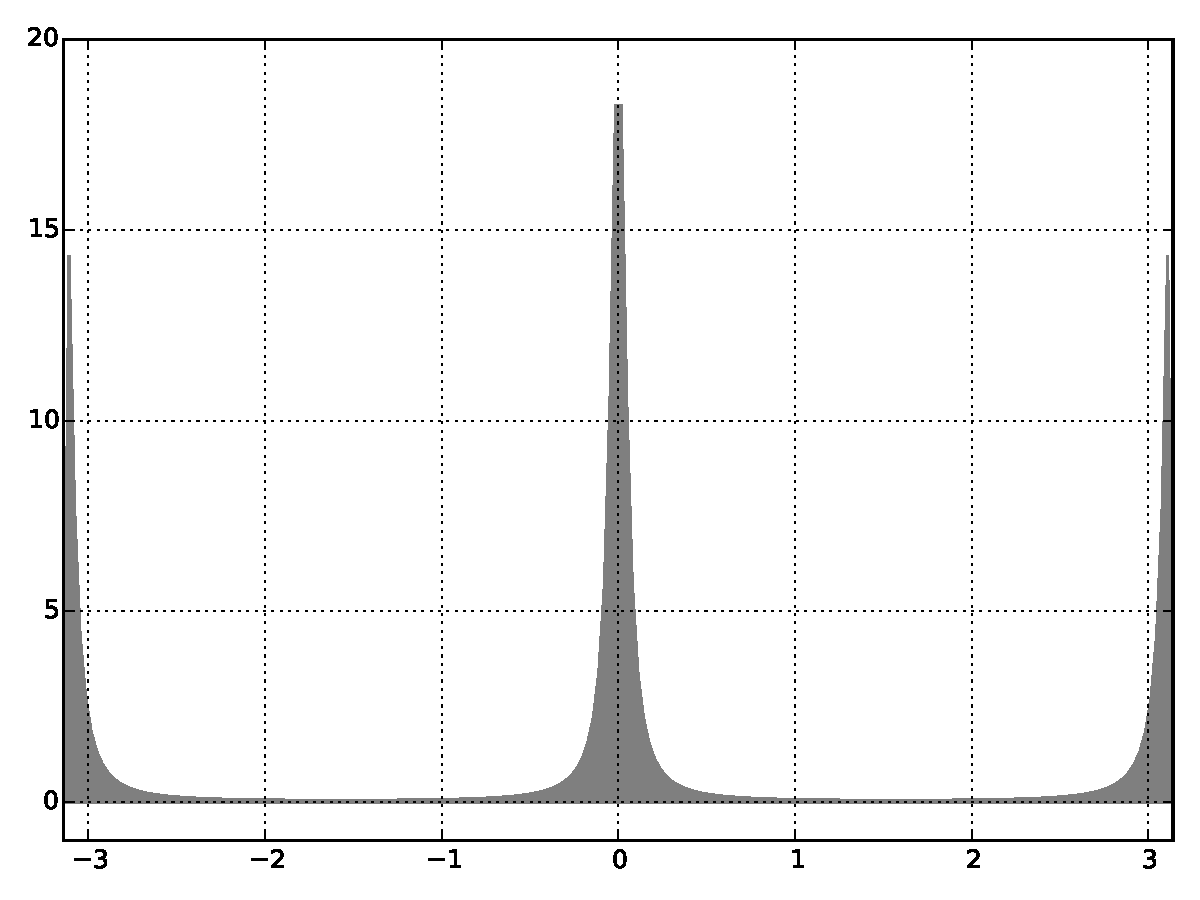
\includegraphics[width=\textwidth]{./images/exact_1D.pdf}
		\caption{Exact}
		\label{fig:exact}
	\end{subfigure}
	\begin{subfigure}{0.3\textwidth}
		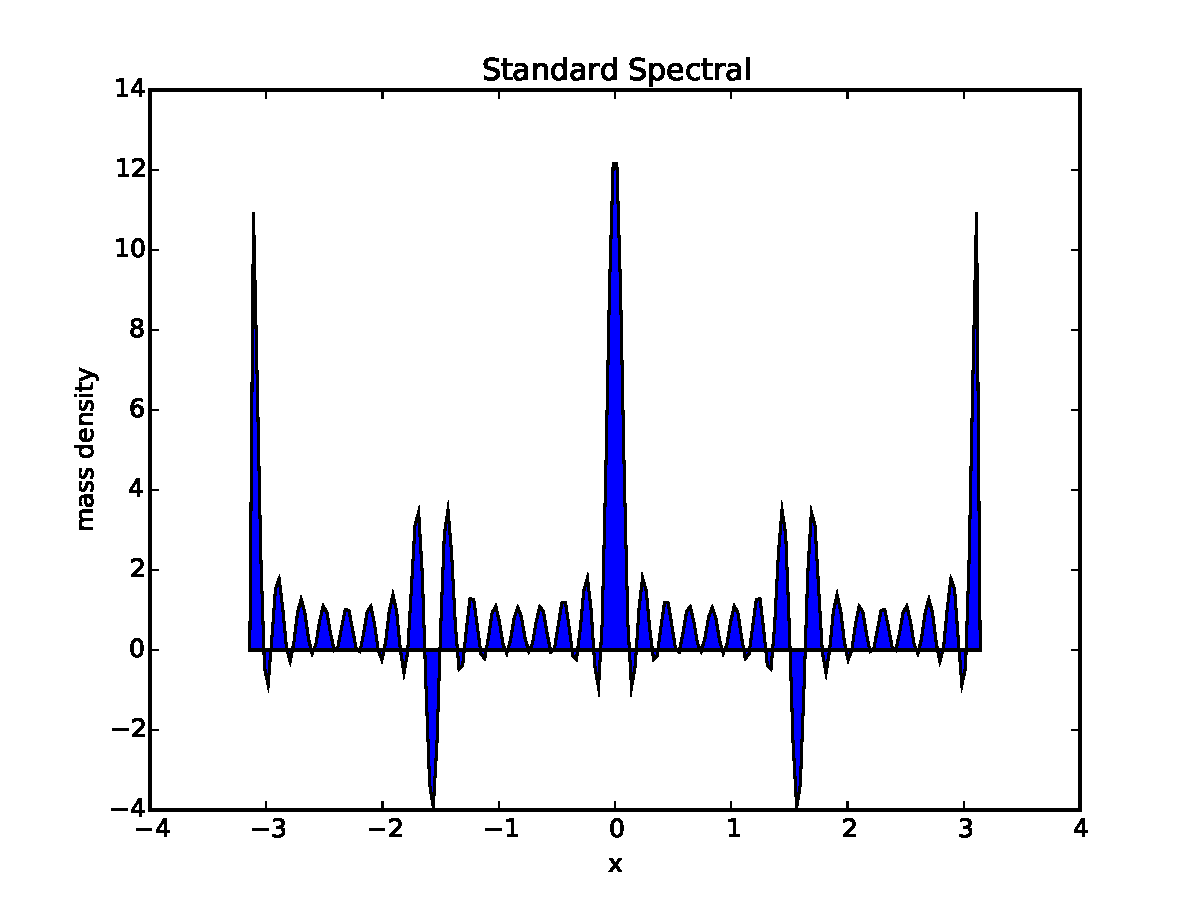
\includegraphics[width=\textwidth]{./images/standard_spectral_1D.pdf}
		\caption{Standard spectral}
		\label{fig:standard spectral}
	\end{subfigure}
	\begin{subfigure}{0.3\textwidth}
		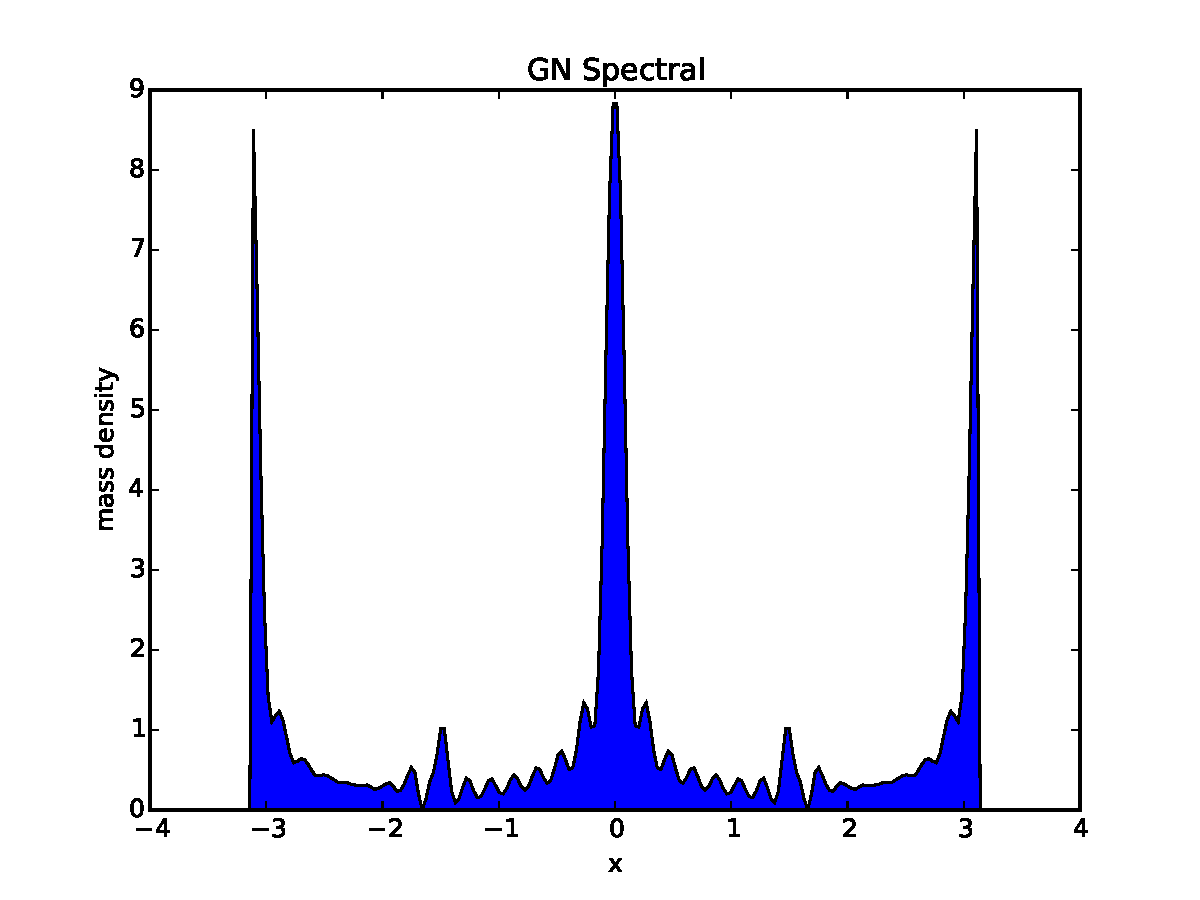
\includegraphics[width=\textwidth]{./images/gn_spectral_1D.pdf}
		\caption{Algorithm \ref{alg:density}}
		\label{fig:gn spectral}
	\end{subfigure}
	\caption{A benchmark computation}
	\label{fig:S1}
\end{figure}

From these figures, it is tempting to suggest that Algorithm \ref{alg:density} has greater qualitative accuracy than a standard spectral discretization.
For one, standard spectral discretization exhibits negative mass, which is not physically achievable in the exact system.
Moreover, the $L^{1}$-norm is not conserved in standard spectral discretization.  However, by Theorem \ref{thm:norms} we know that
the $L^{1}$ norm is conserved in GN discretization.
A plot of the $L^{1}$-norm is given in figure \ref{fig:L1}

\begin{figure}
	\centering
	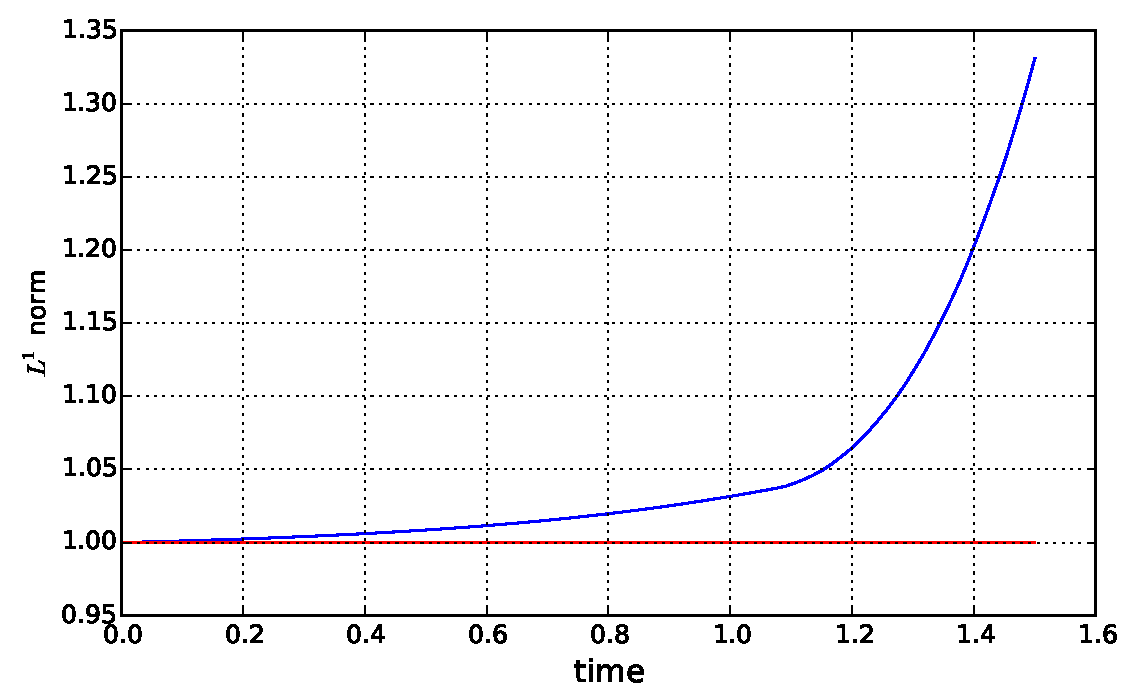
\includegraphics[width=0.8\textwidth]{./images/L1_plot.pdf}
	\caption{A plot of the $L^{1}$-norm vs time.
		The blue line denotes the $L^{1}$ norm under standard spectral discretization.
		The red line denotes the $L^{1}$ norm under Algorithm \ref{alg:density}.
	}
	\label{fig:L1}
\end{figure}

While a Fourier basis is convenient due to our ability to leverage existing fast Fourier transform packages, it is notable that we may use other basis.
In particular, if we consider Daubechies wavelets with mother wavelet that have $4$ vanishing moments, then we may obtain solutions with much greater
accuracy with fewer degrees of freedom. \todo[inline]{Ram should elaborate on this and include some pics.}
At low resolutions, wavelet based solutions come at some cost in terms of sparsity, but this cost vanishes for large resolutions.

\begin{figure}[h]
	\centering
	
\includegraphics[width=0.2\textwidth]{./images/placeholder}
	\caption{Algorithm \ref{alg:density} in a wavelet basis}
\end{figure}


We also know the evolution for an initial function, $f_{0}(x)$.
For example, if $f_{0}(x) = \sin(x)$ then the solution to \eqref{eq:function pde} under this vector-field is
\begin{align}
	f(x;t) = \frac{ e^{-2t} \sin(x) }{ \sqrt{ \cos^{2}(x) + e^{-4t} \sin^{2}(x) } }.
\end{align}

Unfortunately, Algorithm \ref{alg:function} outputs $f$ as an operator on half-densities, and it is not clear how best to invert the hat-map.
However, we can obtain one estimate by applying $\hat{f}_{n}$ to the half-density $\sqrt{dx}$, and then divide the result by $\sqrt{dx}$.
The resulting function appears to approximate $f(x;t)$ well in the flat areas, and overshoot at the peaks.
In comparison, a standard spectral discretization seems to have large spurious oscillations in the center.
These estimates are plotted alongside the exact solution in figure \ref{fig:function}.
We should note that our means of converting $\hat{f}_{n}$ into a function is probably not the best choice of a left inverse to the hat-map.
Different choices yield different approximations to $f(x;t)$, some
of which get the peaks correct, but do poorly in the valleys.

We can see that the operator-norm behaves well using Algorithm \ref{alg:function}.
The operator-norm is conserved to machine precision for Algorithm \ref{alg:function}, while it will drift using standard discretization.

\begin{figure}[h!]
	\centering
	\begin{subfigure}{0.45\textwidth}
		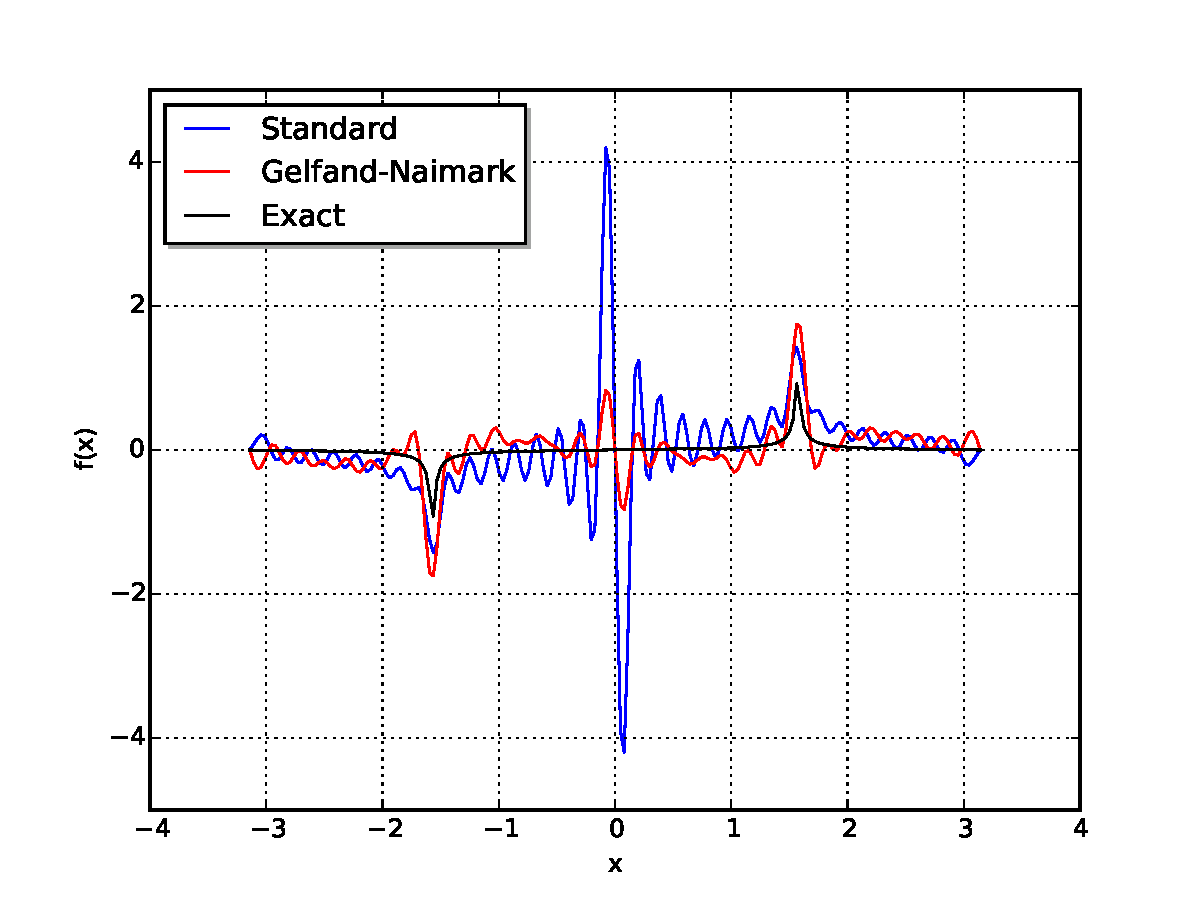
\includegraphics[width=\textwidth]{./images/function_comparison.pdf}
		\caption{Functions}
		\label{fig:function}
	\end{subfigure}
	\begin{subfigure}{0.45\textwidth}
		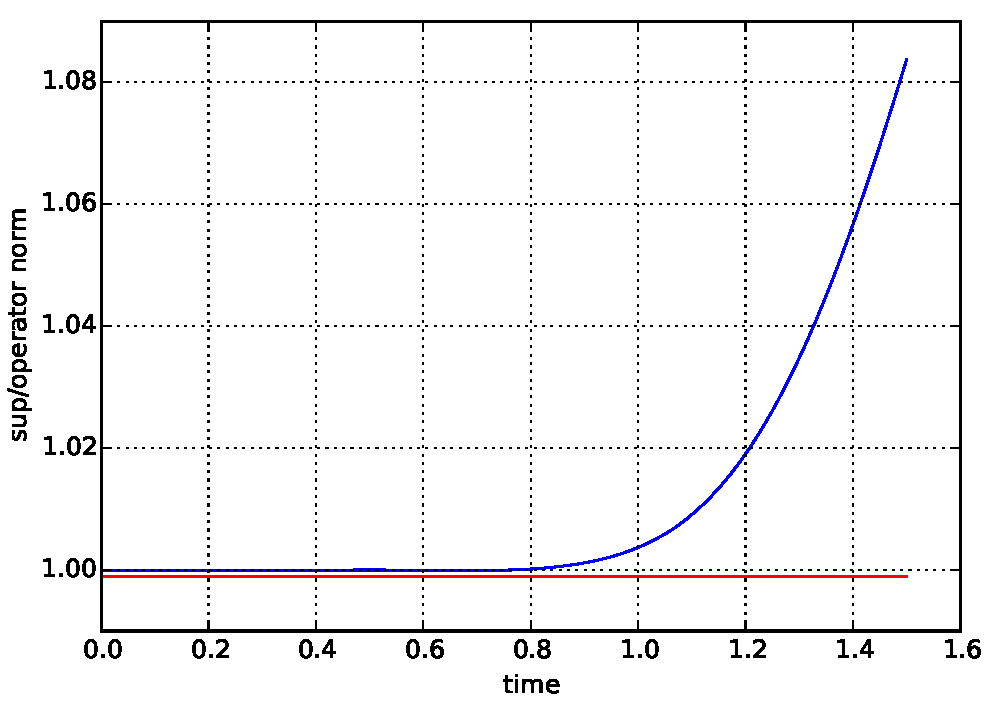
\includegraphics[width=\textwidth]{./images/L_inf_plot.pdf}
		\caption{Operator norms}
		\label{fig:sup norm}
	\end{subfigure}
	\caption{Numerical results for a one-dimensional system}
\end{figure}


\subsection{A system on the 2-torus}
Let us consider the system on $\mathbb{T}^{2}$ given by 
\begin{align}
	\dot{x} &= \cos(2\pi y) - D \sin(2\pi x) \\
	\dot{y} &= -\sin(2 \pi x) - D \cos(2 \pi y).
\end{align}
This can be seen as a dissipative Hamiltonian system with Hamiltonian $H(x,y) = \sin(2 \pi y) - \cos(2 \pi x)$ and dissipation $\vec{F} = D \cdot \nabla H$.
When $D=0$, we have an integrable system and volume is preserved with respect to the standard volume form on $\mathbb{T}^{2}$.
When $D>0$ the system exhibits phase space contraction near minima of $H$ and phase space expansion near the maxima of $H$.
In particular, there are four equilibria $(0, \frac{1}{4}) , (0, \frac{3}{4}) , (\frac{1}{2} , \frac{1}{4} ) , (\frac{1}{2} , \frac{3}{4})$.

In Figure \ref{fig:2 torus} we depict the result of solving \eqref{eq:density pde} using three methods: Algorithm \ref{alg:density}, Monte-Carlo, and a standard spectral discretization.
The top row depicts the result from applying algorithm 2 with the Fourier basis $\{ e^{2\pi i (k_{1}x +k_{2}y)} \mid -8 \leq k_{1},k_{2} \leq 8\}$.
This is a total of $289$ basis functions. 
The middle row depicts the results of a Monte-Carlo simulation with $10^{5}$ particles.
Finally, the bottom row depicts the results of a standard spectral scheme using the same basis as mentioned earlier.
The Monte-Carlo simulation can serve us as a benchmark.
We see that spurious oscillations will manifest using standard discretization, just as in the one-dimensional case.
Also as before, our Algorithm \ref{alg:density} will conserve mass while the standard spectral scheme will diffuse and even negate mass.
By inspection, it appears the largest unstable mode of the standard spectral algorithm is a function with rapid spatial oscillations.
The dominance of this function can be seen visually at time $0.6$ in figure \ref{fig:2 torus}.

\begin{figure}[h!]
	\centering
	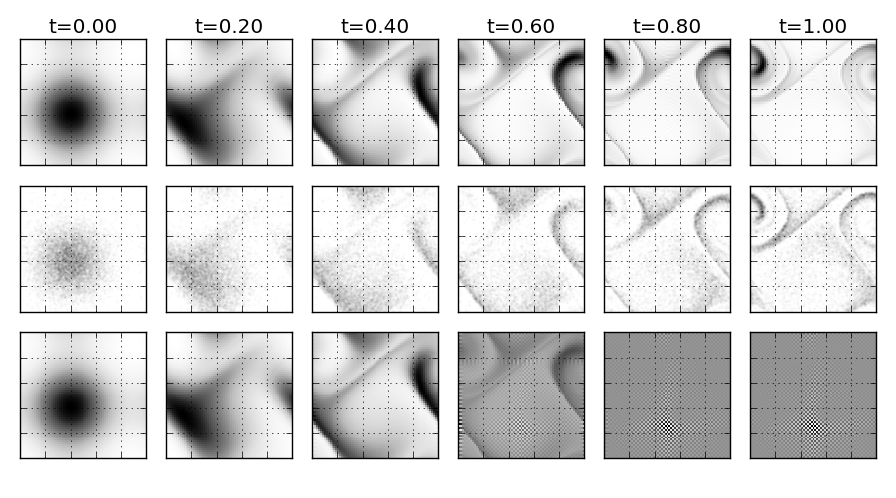
\includegraphics[width=0.8\textwidth]{./images/two_torus.png}
	\caption{ \tiny {\bf Top:} Algorithm \ref{alg:density}, {\bf Middle:} Monte Carlo, {\bf Bottom:} Standard Spectral}
	\label{fig:2 torus}
\end{figure}

Even at dimension $d=2$ Algorithm \ref{alg:function} becomes troublesome, although still feasible.
Instead we implement Algorithm \ref{alg:function2}, which is nothing but a combination of the method of characteristics and a Fourier collocation.
Using the initial function $f_{0}(x,y) = \sin(2\pi y)$ we observe the numerical results shown in Figure \ref{fig:psuedo}

\begin{figure}[h!]
	\centering
	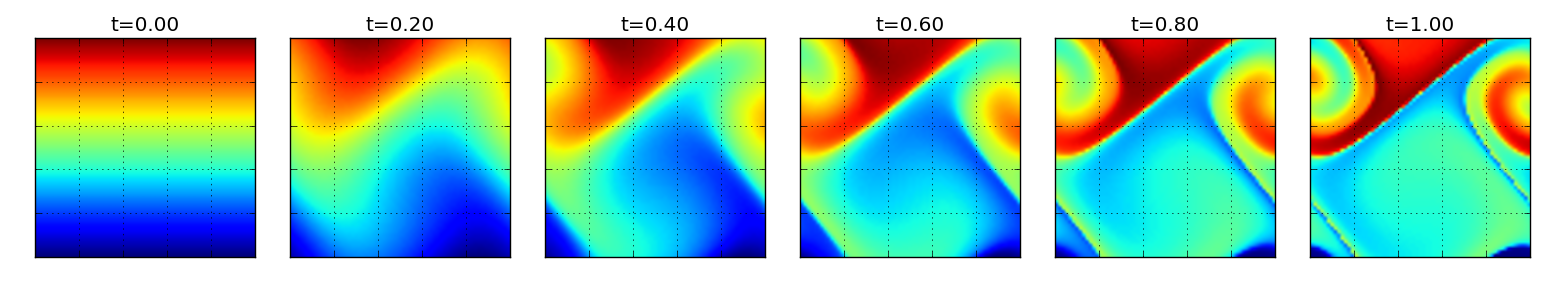
\includegraphics[width=0.7\textwidth]{./images/psuedo_spec_Koopman.png}
	\caption{The result of Algorithm \ref{alg:function2} with initial condition $f_{0}(x,y) = \sin(2\pi y)$.}
	\label{fig:psuedo}
\end{figure}

We can take the inner-product of a density the function output by our respective algorithms.
This inner-product is constant in time for exact solutions to the pdes.
For our numerical solutions these inner-products drift.
However, there is substantially greater drift and variation when using a standard spectral discretization.
These results are shown in Figure \ref{fig:inner}. 
\begin{figure}[h!]
	\centering
	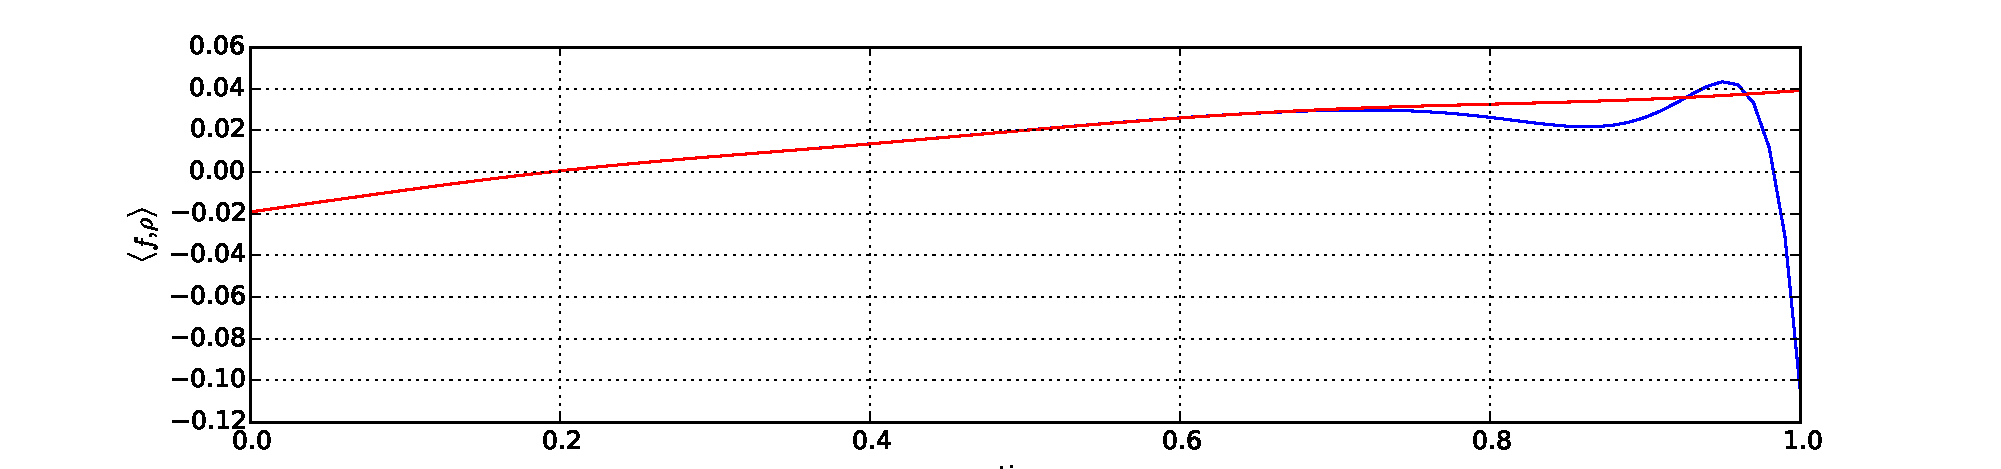
\includegraphics[width=0.7\textwidth]{./images/inner_product_plot.pdf}
	\caption{The inner product between numerically densities and functions.  Blue depicts standard spectral discretization, red depicts the results from Algorithm \ref{alg:density}.}
	\label{fig:inner}
\end{figure}


\subsection{A modified ABC flow}
Consider the system on $\mathbb{T}^{3}$
\begin{align}
	\dot{x} = A \sin( 2\pi z) + C \cos(2\pi y)  + D \cos(2\pi x)\\
	\dot{y} = B \sin( 2\pi z) + A \cos(2\pi y)  + D \cos(2\pi y)\\
	\dot{z} = A \sin( 2\pi z) + B \cos(2\pi y)  + D \cos(2\pi z)\\
\end{align}
For constants $A,B,C,D \in \mathbb{R}$.  When $D=0$ this system is a well studied volume conserving system known as an ABC flow.
When $A > B > C > D = 0$ and $C << 1$, then the solutions to this ODE are chaotic, with a uniform steady state distribution \cite{MajdaBertozzi2002}.
When $D=0$ the operator $\pi(X)$ is identical to the operator $\partial_{\alpha}( \rho X^{\alpha})$ which appears in equation \eqref{eq:density pde},
and Algorithm \ref{alg:half density} will not differ from a standard spectral discretization.\footnote{This is generically the case for any volume conserving system.  The benefits of our algorithm are not as strong in such cases.}
Therefore we will demonstrate the case where $D > 0$ and these discretization are different.
When $D> 0$ volume is no longer conserved and there is a non-uniform steady-state distribution.

Given any probability distribution on $\mathbb{R}^{3}$ we can get a probability distribution on $\mathbb{T}^{3}$ by wrapping it around.
That is to say for any $p \in L^{1}(\mathbb{R}^{3})$ we can consider the probability distribution on $\tilde{p} \in L^{1}(\mathbb{T}^{3})$ implicitly given by
\begin{align*}
	\int_{A} \tilde{p}( {\bf x} ) = \sum_{ {\bf k} \in \mathbb{Z}^{3} } \int_{A + {\bf k} } p( {\bf x} + {\bf k} ).
\end{align*}
for any Borel set $A \subset \mathbb{T}^{3}$ where we view $\mathbb{T}^{3}$ as a unit-cube with boundaries identified.

In particular, let
\begin{align}
	p(x,y,z) = \frac{1}{ (\sigma_{x} \sigma_{y} \sigma_{z} )\sqrt{ 2\pi } } e^{ - \frac{1}{2} ( (x/\sigma_{x})^{2} + (y/\sigma_{y})^{2} +  (z/\sigma_{z})^{2} )}
\end{align}
with $\sigma_{x} = 0.2, \sigma_{y} = 0.3, \sigma_{z} = 0.3$.
We take the resulting wrapped distribution $\tilde{p}$ on $\mathbb{T}$ as an initial conditions to \eqref{eq:density pde}.
Then numerically solve \eqref{eq:density pde} using Algorithm \ref{alg:density}, Monte-Carlo, and a standard spectral method respectively.
The results of applying three different algorithms are shown in figure \ref{fig:ABCD} where we only plot the shadow onto the XY-plane.
The top row depicts the results from using Algorithm \ref{alg:density}.
The middle row depicts the results from using a Monte-Carlo method with $15^{3} = 3375$ particles.
The Monte-Carlo method serves as a good benchmark for the purpose of visual inspection.
Finally, the bottom row depicts the results from using a direct Fourier based discretization of \eqref{eq:density pde}.
Again we see that Algorithm \ref{alg:density} performs quite well.


\begin{figure}
	\centering
	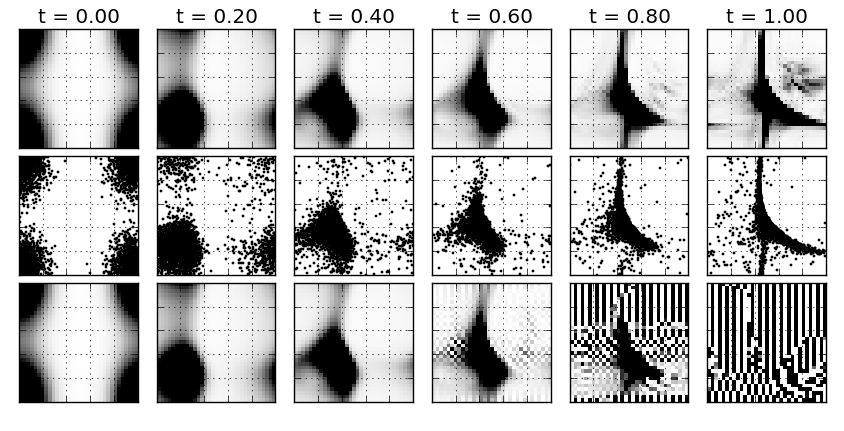
\includegraphics[width=0.8\textwidth]{./images/ABCD_flow.png}
	\caption{ \tiny {\bf Top:} Algorithm \ref{alg:density}, {\bf Middle:} Monte Carlo, {\bf Bottom:} Standard Spectral}
	\label{fig:ABCD}
\end{figure}


\section{Insights from operator theory}

In this section we describe ``why these algorithms work'' from a different perspective, that of Operator theory.
Admittedly, this section is not crucial for a practitioner to benefit from the paper.
Uninterested readers are free to skip it without consequence.
Nonetheless, we consider the following informal discussion valuable from the perspective of research, and integration within the larger mathematics community.
For the sake if pace we will provide references for theorems and claims made in this section, rather than proving them here.

To begin, let us review some definitions.
\begin{defn}
	A \emph{Banach-algebra} is a Banach space, $A$, which is also equipped with a multiplication-like operation $(a,b) \in A \times A \mapsto ab \in A$
	which is bounded and associative in that $\| ab \| \leq \|a \| \|b \|$ and $(ab)c = a(bc)$ for any $a,b,c \in A$.
	
	A \emph{$C^{*}$-algebra} is a Banach algebra, $A$, over the field $\mathbb{C}$ with an involution ``$a \in A \mapsto a^{*} \in A$'' which satisfies
	\begin{align}
		(ab)^{*} = b^{*} a^{*} \\
		(\lambda a)^{*} = \bar{\lambda} a^{*} \\
		\| a \| = \| a^{*}\|.
	\end{align}
	for all $a,b \in A$ and $\lambda \in \mathbb{C}$.
	We call $A$ \emph{unital} if $A$ has a multiplicative identity.
	We call $A$ commutative if $ab = ba$ for all $a,b \in A$.
	
	Finally, a map $T:A \to A$ is called a $*$-automorphism if $T$ is a bounded linear automorphism that preserves products, i.e. $T(ab) = T(a) T(b)$.
	We denote the space of $*$-automorphisms of $A$ by $\operatorname{Aut}(A)$.
\end{defn}

The notion of a $C^{*}$-algebra may appear abstract so we provide the two most important examples.

\begin{example}
	Let $X$ be a topological space.  Then the space of complex valued continuous functions with compact support, $C_{0}(X;\mathbb{C})$, is a $C^{*}$-algebra under the sup-norm and addition/multiplication operations of functions.
	In fact $C_{0}(X;\mathbb{C})$ is a commutative $C^{*}$-algebra.  If $X$ is compact, then the constant function $f(x) = 1$ serves as a multiplicative identity, and this algebra becomes unital.
\end{example}

\begin{example}
	Let $\mathcal{H}$ be a complex Hilbert space. Then the space of bounded operators on $\mathcal{H}$, denoted $B(\mathcal{H})$, is a (non-commutative) $C^{*}$-algebra.
\end{example}

While the notion of a general $C^{*}$-algebras is, apriori, more abstract than the examples above, this feeling of abstraction is an illusion.
One of the cornerstones of operator theory is that \emph{all} $C^{*}$-algebras are contained within these examples.
This is formally given by

\begin{thm}[The Gelfand-Naimark Theorem \cite{GelfandNaimark1943}] \label{thm:GN1}
	Any $C^{*}$-algebra is isomorphic to a sub-algebra of $B(\mathcal{H})$ for some Hilbert space, $\mathcal{H}$.
\end{thm}

For commutative $C^{*}$-algebras more can be said.
In particular we can consider the space of character as in \cite{Bondia2001}.

\begin{defn}
	A \emph{character} of a $C^{*}$-algebra, $A$, is an element of the dual space $x \in A^{*}$ such that
	$x(ab) = x(a) x(c)$.  We denote the space of characters by $X_{A}$.
	The map $A \to X_{A}$ is known as the \emph{Gelfand transform}.
\end{defn}

\begin{prop}[Lemma 1.1 \cite{Bondia2001}]
	If we equipp $A^{*}$ with the weak topology, the space $X_{A} \subset A^{*}$ is a compact Hausdorff space with respect to the relative topology.
\end{prop}
\begin{proof}
	We provide a sketch of the proof.
	One can verify that any character $x \in X_{A}$ is of unit norm.
	Compactness follows from the Banach-Alaoglu theorem.
\end{proof}

For example, if $A$ is a space of continuous complex functions on a manifold $M$, then $X_{A}$ is the space of Dirac-delta distributions, which is homeomorphic to $M$ itself.
The following is really a corollary to \ref{thm:GN1}.

\begin{thm}[The second Gelfand-Naimark Theorem \cite{GelfandNaimark1943}] \label{thm:GN2}
	Any commutative $C^{*}$-algebra is isomorphic to $C(X_{A} ; \mathbb{C})$.
\end{thm}

Historically, theorems \ref{thm:GN1} and \ref{thm:GN2} have been valued because they turn abstract $C^{*}$-algebras into relatively concrete things, such as linear operators or continuous functions.
In this paper, we appear to have gone the other direction.
The map $f \in C(M) \to \hat{f} \in B( L^{2}(M) )$ is \emph{the inverse of the Gelfand transform}!
In particular, correspondence theorem \ref{thm:quantize} is simply the correspondence between advection pdes on $M$ and various odes on $L^{2}(M)$ and $B(L^{2}(M))$ under the Gelfand transform.
Perhaps one of the reasons our algorithms were not done earlier, is because it is not intuitively a good idea to use the Gelfand transform to turn ``concrete'' objects into ``abstract'' ones like this.
However, ``abstract'' does not mean easier to deal with numerically.
In fact, it appears that the abstract characterization is easier to numerically discretize when it comes to advection pdes.
As we have seen, it is easier to represent conservation laws for advection in this form.
In essence this is related to the following corollary of Theorem \ref{thm:GN2}

\begin{cor}[see Corollary 1,7 of \cite{Bondia2001}]
	If $A$ is a commutative $C^{*}$-algebra, and $T:A\to A$ is $*$-automorphism such that $T(a)T(b) = T(ab)$,
	then there is a unique homeomorphism $\Phi_{T} \in \Diff_{0}(X_{A})$
	such that $\Phi_{T}(x) (a) = T^{-1}(a)$.
	In other words, $\Diff_{0}(X_{A}) \equiv \operatorname{Aut}(A)$ as a topological group.
\end{cor}

Said more plainly, any bounded and invertible transformation of $C(M)$ that preserves sums and products is necessarily a homeomorphism.
Thus, conservation of sums of products is more than just a fundamental property of advection.
\emph{Conservation of sums and products is the defining property of advection}.
Consequently, numerical schemes that respect these conservation laws are targeting the defining property of \eqref{eq:function pde} and \eqref{eq:density pde}.
The methods presented in this article provide a case in point, as do particle methods.
In particular, particle methods take $M$ as the fundamental object to use for discretization.
As discussed in the introduction, particle methods conserve (a discrete notion of) sums and products, and therefore we can consider them qualitatively accurate.
The spectral methods considered in this article considers the commutative $C^{*}$-algebra, $C(M)$ as fundamental.
By Theorem \ref{thm:GN2}, the space $C(M)$ has the same data as $M$ itself.
Moreover, by theorem \ref{thm:GN1} we can view $C(M)$ as a space of operators without any loss in data.
As a result, the spectral methods in this paper can be seen as a reasonable discretization one would apply to from the perspective of $C^{*}$-algebras,
while particle methods can be seen as a reasonable discretization one would apply, after using the Gelfand transform.


\section{Conclusion}

\subsection{Future work}

\todo[inline]{Boundary conditions, non-compact mfds}

\subsection{Acknowledgements}

\todo[inline]{Peter Michor, Stephen Marsland, Stefan Sommer,Dmitry Pavlov, Tilak Ratnanather.}

\appendix

\section{Proof that $\pi$ is bracket preserving} \label{app:Lie}
Here we prove that $\pi$ is a Lie algebra morphism.

\section{A perturbed Gronwall's inequality}
\begin{lem} \label{lem:Gronwall}
If $\frac{du}{dt} \leq Ku + \epsilon$ then $u(t) \leq (\epsilon t + u(0) ) e^{Kt}$.
\end{lem}
\begin{proof}
	Let $w (t)= u (t) e^{-Kt}$.  Then for $t \geq 0$ we find
	\begin{align}
		\frac{dw}{dt} = \frac{du}{dt} e^{-Kt} - K w \leq (Ku+\epsilon) e^{-Kt} - Kw = \epsilon e^{-Kt} \leq \epsilon
	\end{align}
	Thus $w(t) \leq \epsilon t + w(0) = \epsilon t + u(0)$.
\end{proof}

\bibliographystyle{amsalpha}
\bibliography{hoj.bib}
\end{document}
